\documentclass[11pt]{article}

\usepackage[margin=1in]{geometry}
\usepackage{amsmath}
\usepackage{amssymb}
\usepackage{graphicx}
\usepackage{booktabs}
\usepackage{array}
\usepackage{microtype}
\usepackage{hyperref}

\newcommand{\dd}{\mathrm{d}}
\newcommand{\gdet}{\sqrt{\gamma}}
\newcommand{\I}{I}
\newcommand{\nhat}{\hat{n}}
\newcommand{\adm}{\mathrm{ADM}}
\newcommand{\cks}{\mathrm{CKS}}
\newcommand{\ud}{\mathrm{d}}
\newcommand{\nuE}{\nu_{\rm E}}
\newcommand{\nucm}{\nu_{\rm cm}}
\newcommand{\code}[1]{\texttt{#1}}

\title{\bfseries Dynamical-Spacetime Discrete-Ordinates Radiation in AthenaK}
\author{Circumbinary radiation implementation draft}
\date{\today}

\begin{document}

\maketitle

\begin{abstract}
We describe a standalone discrete-ordinates radiation module for AthenaK that
can evolve radiation on time-dependent ADM backgrounds.  The existing radiation
solver is tied to stationary Cartesian Kerr-Schild metrics: it stores a signed
Killing-energy-normalized intensity, uses metric-dependent angular drift
coefficients that can be precomputed, and is therefore efficient for isolated
stationary black holes.  These assumptions are not appropriate for binary black
hole backgrounds or for metric data supplied by a dynamical spacetime solver.
The new \code{dyn\_radiation} module keeps a CKS compatibility mode for
stationary-solver regression tests, but adds an ADM formulation in which the evolved
quantity is the Eulerian densitized intensity, the spatial transport speed is
\(\alpha s^i-\beta^i\), angular geodesic advection is computed from the ADM
Hamiltonian, and the geometric energy source is written in Valencia form using
\(\alpha\), \(\beta^i\), \(\gamma_{ij}\), and \(K_{ij}\).  This avoids assuming a
time-independent metric and does not require explicit gauge-field time
derivatives beyond the ADM metric-evolution relation for
\(\partial_t\gamma_{ij}\).  The per-angle ADM metric source is applied through
the closed-form exponential stage increment for the local multiplicative
source.  In the present implementation the radiation field is metric-passive:
it is transported on ADM/Z4c geometry, but its stress-energy is not included in
the Z4c metric right-hand side.  We also add a diagnostic null-geodesic
particle pusher for beam-edge tracers on ADM backgrounds.  Flat-space beam tests
reproduce the legacy solver to roundoff, radiation-hydrodynamic linear-wave
tests reproduce the legacy error norms in stationary Kerr-Schild mode, and a
superposed boosted-Kerr-Schild binary test exercises the ADM beam source, ADM
matter coupling, and null-particle tracers.
\end{abstract}

\noindent\textbf{Keywords:} numerical relativity; radiation hydrodynamics;
general relativistic radiation transport; binary black holes; AthenaK

\section{Introduction}
\label{sec:introduction}

Radiation transport in relativistic accretion flows is usually implemented on a
fixed analytic background.  For a single Kerr black hole this is a good
approximation in many applications: the metric is stationary, the coordinate
tetrad can be generated once, and the angular advection terms that bend rays in
momentum space can be precomputed.  Circumbinary and dynamical-spacetime
applications remove these simplifications.  The lapse, shift, spatial metric,
and extrinsic curvature may change in time; the background may be supplied by a
numerical relativity evolution; and the same radiation module should be usable
with superposed black-hole data, Z4c data, or any other ADM source.

The goal of the implementation described here is narrower than a full
production radiation scheme.  We add a separate \code{dyn\_radiation} package,
rather than changing the existing \code{radiation} module, so that the legacy
stationary path remains available and bitwise comparisons remain possible.  The
current ADM branch implements spatial transport, angular geodesic advection,
radiation-matter coupling, and the radiation energy source in a
Valencia-compatible form.  The angular advection coefficients are rebuilt from
cached ADM geometry each stage, so ADM mode now supports
\code{angular\_fluxes=true}.  Radiation is deliberately one-way coupled to the
metric in this pass: the metric can affect radiation through the ADM fields,
but radiation does not source the Z4c evolution.  The implementation remains
separate from the legacy solver so stationary CKS behavior can still be tested
directly.

The paper is organized as follows.  Section~\ref{sec:notation} fixes notation
and derives the radiation variables from the invariant distribution function.
Section~\ref{sec:legacy} summarizes the stationary-metric solver.
Section~\ref{sec:adm} derives the ADM variables, geometric source terms, and
angular geodesic operator used by the new solver.  Section~\ref{sec:alg}
describes the numerical algorithm and implementation.  Section~\ref{sec:null}
documents the null-particle beam-edge diagnostic.  Section~\ref{sec:tests}
presents the regression and smoke tests.  Section~\ref{sec:checklist}
summarizes direct consistency checks.  Section~\ref{sec:discussion} summarizes
limitations and next implementation steps.

\section{Conventions and Radiation Variables}
\label{sec:notation}

We use units with \(c=G=1\) and metric signature \((-+++) \).  Greek indices
\(\mu,\nu,\ldots\) run over spacetime components \(0,1,2,3\), Latin indices
\(i,j,\ldots\) run over spatial components \(1,2,3\), and hatted Latin indices
\(\hat a,\hat b,\ldots\) denote an orthonormal spatial tetrad.  Repeated
indices are summed.  The radiation module is grey: it evolves intensity
integrated over photon frequency, but still resolves propagation direction on
a discrete angular grid.

The invariant starting point is the photon distribution function \(f(x^\mu,p_i)\)
on the null mass shell.  In vacuum, Liouville's theorem says that \(f\) is
constant along null geodesics:
\begin{equation}
  \frac{\dd f}{\dd \lambda}
  =
  p^\mu\frac{\partial f}{\partial x^\mu}
  +\frac{\dd p_i}{\dd \lambda}\frac{\partial f}{\partial p_i}
  =0,
  \label{eq:liouville}
\end{equation}
where \(\lambda\) is an affine parameter and \(p_\mu\) is the photon covector.
Matter interaction adds an invariant collision term to the right-hand side.
For a local orthonormal observer measuring photon frequency \(\nu\), the
frequency-dependent specific intensity satisfies
\begin{equation}
  \frac{I_\nu}{\nu^3} \propto f .
\end{equation}
After integrating over frequency, the bolometric grey intensity transforms as
\begin{equation}
  I \propto \nu^4 f .
  \label{eq:bolometric_transform}
\end{equation}
This is why the matter-coupling kernel converts Eulerian-frame intensity to
fluid-comoving intensity with a fourth power of the frequency ratio.

The angular grid stores a finite set of unit directions
\(\ell_n^{(\hat a)}\) and quadrature weights \(w_n\), with
\begin{equation}
  \ell_n^{(\hat a)}\ell_{n(\hat a)}=1,\qquad
  \sum_n w_n \simeq 4\pi .
\end{equation}
The continuum angular integrals are approximated by these quadrature sums.
The code variable \(U_n\) is not the invariant distribution function itself; it
is a finite-volume conserved density whose precise normalization depends on
the metric formulation.  The CKS compatibility path keeps the historical signed
stationary-metric normalization.  The ADM path uses the Eulerian volume density
\(U_n=\sqrt{\gamma}I_n\), derived below.

\section{Stationary-Metric Radiation Solver}
\label{sec:legacy}

The existing AthenaK radiation package evolves grey specific intensity on a set
of angular bins.  For each angular bin \(n\), a local orthonormal tetrad
direction is
\begin{equation}
  q^{(\hat{\alpha})}_n = (1,\ell_n,m_n,p_n), \qquad
  \ell_n^2 + m_n^2 + p_n^2 = 1 .
\end{equation}
The stationary Cartesian Kerr-Schild (CKS) tetrad maps this direction to a
coordinate null vector,
\begin{equation}
  k^\mu_n = e_{(\hat{\alpha})}^{\ \mu} q^{(\hat{\alpha})}_n,
  \qquad
  k_{\mu,n}=g_{\mu\nu}k^\nu_n .
\end{equation}
For a stationary metric, the positive photon Killing energy is
\(-k_\mu(\partial_t)^\mu=-k_0\) for the \((-+++)\) signature used here.  The
legacy finite-volume variable stores the signed covariant time-component
normalization,
\begin{equation}
  U_n = k^0_n k_{0,n}\I_n ,
  \label{eq:legacyU}
\end{equation}
and the reconstructed primitive entering the spatial flux is
\begin{equation}
  k_{0,n}\I_n = \frac{U_n}{k^0_n}.
\end{equation}
The corresponding spatial flux in direction \(i\) is
\begin{equation}
  F^i_n = k^i_n k_{0,n}\I_n .
  \label{eq:legacy_flux}
\end{equation}
Thus the coordinate transport speed of the legacy conserved variable is
\(F^i_n/U_n=k^i_n/k^0_n\), while \(k_0\) itself is only the covariant time
component; \(-k_0\) is the positive Killing energy.
Ignoring matter coupling for the moment, the schematic update is
\begin{equation}
  \partial_t U_n + \partial_i F^i_n
  + \nabla_\Omega\cdot A_n = S_n ,
  \label{eq:legacy_update}
\end{equation}
where \(A_n\) is the angular-space flux induced by geodesic bending.  In the
stationary CKS module the tetrad, angular face maps, and angular drift
coefficients are precomputed.  This is efficient and accurate on a fixed black
hole background, but it encodes the assumptions that the metric is known
analytically, stationary, and tied to the CKS tetrad construction.

\section{ADM Formulation for Dynamical Backgrounds}
\label{sec:adm}

\subsection{ADM split and Eulerian observers}

The dynamical branch uses the standard ADM line element
\begin{equation}
  \dd s^2 =
  -\alpha^2 \dd t^2
  +\gamma_{ij}(\dd x^i+\beta^i\dd t)(\dd x^j+\beta^j\dd t),
  \label{eq:adm_metric}
\end{equation}
where \(\alpha\) is the lapse, \(\beta^i\) is the shift, and
\(\gamma_{ij}\) is the spatial metric.  The Eulerian normal observer has
\begin{equation}
  n^\mu=\left(\frac{1}{\alpha},-\frac{\beta^i}{\alpha}\right),
  \qquad
  n_\mu=(-\alpha,0,0,0).
\end{equation}
The determinant of the spatial metric is denoted \(\gamma\), so the proper
spatial volume element is \(\sqrt{\gamma}\,\dd^3x\).

The radiation tetrad timelike leg is chosen to be the Eulerian observer,
\begin{equation}
  e_{(\hat{0})}^{\ \mu}=n^\mu ,
\end{equation}
and define spatial tetrad columns \(E_{(\hat{a})}^{\ i}\) satisfying
\begin{equation}
  e_{(\hat{a})}^{\ \mu}=(0,E_{(\hat{a})}^{\ i}),
  \qquad
  \gamma_{ij}E_{(\hat{a})}^{\ i}E_{(\hat{b})}^{\ j}
  = \delta_{\hat{a}\hat{b}} .
  \label{eq:spatial_tetrad}
\end{equation}
The dual spatial co-triad is \(e^{(\hat a)}_{\ i}\), with
\begin{equation}
  e^{(\hat a)}_{\ i}E_{(\hat b)}^{\ i}=\delta^{\hat a}_{\ \hat b},
  \qquad
  \gamma_{ij}=e^{(\hat a)}_{\ i}e_{(\hat a)j}.
  \label{eq:cotriad_def}
\end{equation}
For angular-bin direction \(\ell_n^{(\hat{a})}\), the Eulerian spatial unit
vector in coordinates is
\begin{equation}
  s^i_n = E_{(\hat{a})}^{\ i}\ell_n^{(\hat{a})},
  \qquad
  \gamma_{ij}s^i_n s^j_n=1 .
  \label{eq:eulerian_direction}
\end{equation}

\subsection{Densitized intensity}

For a photon with Eulerian frequency
\begin{equation}
  \nuE = -n_\mu p^\mu = \alpha p^0 ,
\end{equation}
write the photon four-momentum as
\begin{equation}
  p^\mu = \nuE(n^\mu+s^\mu), \qquad s^\mu=(0,s^i),
  \label{eq:photon_decomp}
\end{equation}
where \(s^\mu n_\mu=0\) and \(\gamma_{ij}s^is^j=1\).  Equation
\eqref{eq:photon_decomp} immediately gives the coordinate propagation speed
\begin{equation}
  v^i_n=\frac{p^i}{p^0}=\alpha s^i_n-\beta^i .
  \label{eq:admspeed}
\end{equation}

The ADM conserved variable is the Eulerian proper-volume density of grey
intensity,
\begin{equation}
  U_n = \sqrt{\gamma}\,\I_n ,
  \label{eq:admU}
\end{equation}
with spatial flux
\begin{equation}
  F^i_n = \sqrt{\gamma}\,v^i_n\I_n .
  \label{eq:admflux}
\end{equation}
Equations~\eqref{eq:admspeed}--\eqref{eq:admflux} reduce to ordinary flat-space
transport when \(\alpha=1\), \(\beta^i=0\), and
\(\gamma_{ij}=\delta_{ij}\).  They also make the normalization difference from
the legacy solver explicit: ADM mode evolves the volume-weighted intensity
seen by Eulerian observers, not the Killing-energy weighted intensity in
Equation~\eqref{eq:legacyU}.

\subsection{Radiation moments and Valencia equations}

The stress-energy tensor of a grey radiation field can be decomposed relative
to the Eulerian observer as
\begin{equation}
  T_{\rm rad}^{\mu\nu}
  =
  E n^\mu n^\nu
  +n^\mu F^\nu+F^\mu n^\nu
  +P^{\mu\nu},
  \label{eq:rad_tmunu_decomp}
\end{equation}
where \(F^\mu n_\mu=0\) and \(P^{\mu\nu}n_\nu=0\).  In the tetrad quadrature
used by the code,
\begin{align}
  E &= \sum_n w_n \I_n, \\
  F^i &= \sum_n w_n \I_n s^i_n, \\
  P^{ij} &= \sum_n w_n \I_n s^i_n s^j_n ,
  \label{eq:moments}
\end{align}
and \(P^i_{\ j}=P^{ik}\gamma_{kj}\).  These definitions are useful for
verification: summing the discrete per-angle equations must recover the
conservative equations for \(E\) and \(S_i=\gamma_{ij}F^j\).

Starting from stress-energy conservation,
\begin{equation}
  \nabla_\mu T_{\rm rad}^{\mu\nu}=G^\nu ,
  \label{eq:rad_conservation}
\end{equation}
where \(G^\nu\) is the force density on the radiation field.  The force on the
matter is therefore \(-G^\nu\).  With this sign convention, the Eulerian energy
equation is obtained by projecting along \(n_\nu\).  In vacuum
\((G^\nu=0)\), or before applying matter coupling, this gives
\begin{equation}
  \partial_t(\sqrt{\gamma}E)
  +\partial_i\left[\sqrt{\gamma}(\alpha F^i-\beta^iE)\right]
  =
  \sqrt{\gamma}\left(\alpha P^{ij}K_{ij}
  -F^i\partial_i\alpha\right).
  \label{eq:valenciaE}
\end{equation}
Projecting Equation~\eqref{eq:rad_conservation} into the spatial slice gives
the momentum equation
\begin{equation}
  \partial_t(\sqrt{\gamma}S_j)
  +\partial_i\left[\sqrt{\gamma}(\alpha P^i_{\ j}-\beta^iS_j)\right]
  =
  \sqrt{\gamma}\left[
    \frac{1}{2}\alpha P^{ik}\partial_j\gamma_{ik}
    +S_i\partial_j\beta^i
    -E\partial_j\alpha\right].
  \label{eq:valencia_momentum}
\end{equation}
Equations~\eqref{eq:valenciaE} and \eqref{eq:valencia_momentum} are the same
geometric source structure used by Valencia GR hydrodynamics.  Metric time
evolution enters through the ADM identity for \(\partial_t\gamma_{ij}\), with
\(K_{ij}\) supplying the energy-source term and the co-triad time derivative
supplying the angular drift.  This is the central reason the ADM radiation path
is not tied to a stationary gauge.

For a single angular bin, substitute
\[
  E\rightarrow I_n,\qquad
  F^i\rightarrow I_ns^i_n,\qquad
  P^{ij}\rightarrow I_ns^i_ns^j_n .
\]
The per-angle geometric energy source used in the code is therefore
\begin{equation}
  S^{\mathrm{geom}}_n =
  U_n\left(\alpha K_{ij}s^i_ns^j_n
  -s^i_n\partial_i\alpha\right).
  \label{eq:anglesource}
\end{equation}
Summing Equation~\eqref{eq:anglesource} over angles reproduces the right-hand
side of Equation~\eqref{eq:valenciaE}.  The energy source is agnostic to the
gauge condition used to obtain the ADM data and does not require assuming
\(\partial_t \alpha=0\), \(\partial_t\beta^i=0\), or
\(\partial_t\gamma_{ij}=0\).

\subsection{ADM angular geodesic advection}

The angular advection operator accounts for geodesic bending, i.e. the change
of \(\ell^{(\hat a)}\) as a ray moves through a curved or time-dependent
tetrad.  It is derived from the null Hamiltonian.  The inverse ADM metric is
\begin{equation}
  g^{00}=-\frac{1}{\alpha^2},\qquad
  g^{0i}=\frac{\beta^i}{\alpha^2},\qquad
  g^{ij}=\gamma^{ij}-\frac{\beta^i\beta^j}{\alpha^2}.
\end{equation}
The null constraint \(g^{\mu\nu}p_\mu p_\nu=0\) gives
\begin{equation}
  -p_0 = H(x^i,p_i)
  =\alpha \Pi-\beta^ip_i,\qquad
  \Pi=\sqrt{\gamma^{ij}p_ip_j}.
  \label{eq:adm_hamiltonian_full}
\end{equation}
Using coordinate time \(t\) as the evolution parameter, Hamilton's equations
are
\begin{align}
  \dot x^i
  &=\frac{\partial H}{\partial p_i}
    =\alpha\frac{\gamma^{ij}p_j}{\Pi}-\beta^i,\\
  \dot p_i
  &=-\frac{\partial H}{\partial x^i}
    =-(\partial_i\alpha)\Pi
      +p_j\partial_i\beta^j
      -\frac{\alpha}{2\Pi}p_jp_k\partial_i\gamma^{jk}.
  \label{eq:adm_pdot_full}
\end{align}
The code normalizes the momentum by the Eulerian photon energy, so
\(\Pi=1\),
\begin{equation}
  p_i=e^{(\hat a)}_{\ i}\ell_{(\hat a)},\qquad
  s^i=\gamma^{ij}p_j=E^i_{\ (\hat a)}\ell^{(\hat a)}.
\end{equation}
With this normalization, the coordinate speed follows from
Equations~\eqref{eq:adm_hamiltonian_full} and \eqref{eq:adm_pdot_full}.  The
force used to advance the angular direction is the energy-rescaled canonical
force \(A_i=(1/\nu_{\rm E})\,dP_i/dt\) for the unnormalized covariant
momentum \(P_i=\nu_{\rm E}p_i\):
\begin{equation}
  H(x^i,p_i)=\alpha\sqrt{\gamma^{ij}p_i p_j}-\beta^i p_i .
  \label{eq:adm_hamiltonian}
\end{equation}
For the Eulerian tetrad normalization used here,
\(\sqrt{\gamma^{ij}p_i p_j}=1\), \(p_i=e^{(\hat a)}_{\ i}\ell_{(\hat a)}\),
and
\begin{align}
  \dot x^i &= \alpha s^i-\beta^i,\\
  A_i &=
  -\partial_i\alpha+p_j\partial_i\beta^j
  -\frac{\alpha}{2}p_jp_k\partial_i\gamma^{jk}.
  \label{eq:adm_pdot}
\end{align}
The literal derivative of the normalized covector \(p_i=P_i/\nu_{\rm E}\)
differs from \(A_i\) by a component parallel to \(p_i\), which carries the
finite gravitational/Doppler frequency shift.  The angular update below removes
that parallel component and keeps only the tangential drift on the unit sphere.

The angular direction is obtained from the co-momentum through
\begin{equation}
  \ell^{(\hat a)} = E^i_{\ (\hat a)}p_i .
\end{equation}
Differentiating in the same triad gauge gives
\begin{equation}
  \dot\ell^{(\hat a)}
  =E^i_{\ (\hat a)}
  \left[
    A_i
    -\left(\partial_t e^{(\hat b)}_{\ i}
    +\dot x^j\partial_j e^{(\hat b)}_{\ i}\right)\ell_{(\hat b)}
  \right].
  \label{eq:admdotell}
\end{equation}
Any component of \(\dot\ell^{(\hat a)}\) parallel to
\(\ell^{(\hat a)}\) is the frequency/normalization drift of the unconstrained
canonical force, not a physical angular drift on the unit sphere, and is
projected away:
\begin{equation}
  \dot\ell^{(\hat a)}
  \leftarrow
  \dot\ell^{(\hat a)}
  -(\ell_{\hat b}\dot\ell^{(\hat b)})\ell^{(\hat a)} .
  \label{eq:ell_projection}
\end{equation}

The time derivative of the co-triad is obtained by differentiating the same
Cholesky factorization used for the spatial triad, with
\begin{equation}
  \partial_t\gamma_{ij}
  =-2\alpha K_{ij}+D_i\beta_j+D_j\beta_i .
  \label{eq:adm_gdot}
\end{equation}
This relation is an identity in the ADM split and is independent of the
particular gauge condition used to evolve \(\alpha\) and \(\beta^i\).
The implementation uses the equivalent partial-derivative form
\begin{equation}
  \partial_t\gamma_{ij}
  =
  -2\alpha K_{ij}
  +\beta^k\partial_k\gamma_{ij}
  +\gamma_{ik}\partial_j\beta^k
  +\gamma_{jk}\partial_i\beta^k ,
  \label{eq:adm_gdot_partial}
\end{equation}
which makes the shift Lie derivative explicit.

\subsection{Cholesky tetrad gauge and derivatives}

The implementation uses a Cholesky gauge for the spatial tetrad.  Let
\(\gamma_{ij}=L_{i\hat a}L_{j\hat a}\), with \(L\) lower triangular:
\begin{align}
  L_{1\hat1}&=\sqrt{\gamma_{11}},&
  L_{2\hat1}&=\frac{\gamma_{12}}{L_{1\hat1}},&
  L_{3\hat1}&=\frac{\gamma_{13}}{L_{1\hat1}},\\
  L_{2\hat2}&=\sqrt{\gamma_{22}-L_{2\hat1}^2},&
  L_{3\hat2}&=\frac{\gamma_{23}-L_{3\hat1}L_{2\hat1}}{L_{2\hat2}},&
  L_{3\hat3}&=\sqrt{\gamma_{33}-L_{3\hat1}^2-L_{3\hat2}^2}.
\end{align}
The co-triad is \(e^{(\hat a)}_{\ i}=L_{i\hat a}\), and the triad columns are
\(E^i_{\ (\hat a)}=(L^{-T})^i_{\ \hat a}\).  For any derivative operator
\(\partial_q\), where \(q\) may be a spatial coordinate or \(t\), the code uses
the differentiated Cholesky relations
\begin{align}
  \partial_q L_{1\hat1}
    &=\frac{\partial_q\gamma_{11}}{2L_{1\hat1}},\\
  \partial_q L_{2\hat1}
    &=\frac{\partial_q\gamma_{12}
      -L_{2\hat1}\partial_qL_{1\hat1}}{L_{1\hat1}},\\
  \partial_q L_{3\hat1}
    &=\frac{\partial_q\gamma_{13}
      -L_{3\hat1}\partial_qL_{1\hat1}}{L_{1\hat1}},\\
  \partial_q L_{2\hat2}
    &=\frac{\partial_q\gamma_{22}
      -2L_{2\hat1}\partial_qL_{2\hat1}}{2L_{2\hat2}},\\
  \partial_q L_{3\hat2}
    &=\frac{
      \partial_q\gamma_{23}
      -(\partial_qL_{3\hat1})L_{2\hat1}
      -L_{3\hat1}(\partial_qL_{2\hat1})
      -L_{3\hat2}(\partial_qL_{2\hat2})}
      {L_{2\hat2}},\\
  \partial_q L_{3\hat3}
    &=\frac{\partial_q\gamma_{33}
      -2L_{3\hat1}\partial_qL_{3\hat1}
      -2L_{3\hat2}\partial_qL_{3\hat2}}{2L_{3\hat3}}.
  \label{eq:chol_derivatives}
\end{align}
These equations are important for reproducibility: the angular drift uses the
same tetrad gauge as the spatial transport and matter-coupling transforms.

\subsection{Projection to the angular finite-volume grid}

The geodesic angular mesh is a finite-volume mesh on the unit sphere.  Writing
\[
  \ell=(\sin\theta\cos\psi,\sin\theta\sin\psi,\cos\theta),
\]
the tangent angular velocities are
\begin{align}
  \dot\theta &=-\frac{\dot\ell_z}{\sin\theta},\\
  \sin^2\theta\,\dot\psi
    &=\ell_x\dot\ell_y-\ell_y\dot\ell_x .
  \label{eq:theta_psi_dot}
\end{align}
The code projects these two components onto the precomputed angular face
normal stored by the geodesic grid.  The resulting scalar face speed is the
array \(\code{na}\).  In ADM mode \(\code{na}\) is already a coordinate-time
angular velocity, so the angular finite-volume flux upwinds \(U_n\) directly.
In the CKS compatibility branch the historical angular primitive \(U_n/k^0_n\)
is still used, preserving the stationary solver behavior.
The spherical-coordinate expressions are singular at the poles; the
implementation treats them only as a local representation before projection to
geodesic-grid face normals and suppresses the polar singular limit rather than
using a divergent \(\dot\theta\).

\section{Numerical Algorithm and Implementation}
\label{sec:alg}

\subsection{Standalone solver layout}

The new module is intentionally independent of \code{src/radiation}.  It lives
under \code{src/dyn\_radiation} and supports two metric modes:
\begin{description}
  \item[CKS compatibility mode] uses the same normalization and transport
    variables as the legacy solver, enabling direct regression comparisons.
  \item[ADM mode] uses Equations~\eqref{eq:admU}--\eqref{eq:anglesource} and
    obtains \(\alpha\), \(\beta^i\), \(\gamma_{ij}\), and \(K_{ij}\) from the
    active relativistic mesh data.
\end{description}
The solver is constructed as a relativistic component when either the CKS path
or the dynamical ADM path is active.  This is required so that the radiation
state has access to the metric-dependent arrays used by the flux and source
kernels.

For Z4c evolutions the present solver is a test-field radiation system.  The
NR task graph no longer queues a radiation stress-energy task before
\code{Z4c\_CalcRHS}, and \code{Tmunu} storage is not allocated solely because
\code{dyn\_radiation} is enabled.  Matter stress-energy from the MHD/dynGRMHD
path is unchanged.  A run that combines \code{dyn\_radiation} and \code{z4c}
must use \code{geometry=adm}; the CKS mode is retained only for fixed
background compatibility and regression tests.

\subsection{Finite-volume equation actually advanced}

For each angular cell \(n\), ADM mode advances
\begin{equation}
  \partial_t U_n
  +\partial_i\left(\sqrt{\gamma}v_n^i I_n\right)
  +\mathcal{D}_\Omega\left(U_n\dot\ell_n\right)
  =
  S^{\rm geom}_n+C_n ,
  \label{eq:adm_angle_fv}
\end{equation}
where \(U_n=\sqrt{\gamma}I_n\), \(v_n^i=\alpha s_n^i-\beta^i\),
\(\mathcal{D}_\Omega\) is the finite-volume angular divergence on the
geodesic grid, \(S^{\rm geom}_n\) is Equation~\eqref{eq:anglesource}, and
\(C_n\) contains emission, absorption, scattering, and user source terms.  On
a Cartesian mesh cell with coordinate widths \(\Delta x^i\), the explicit
transport part of one Runge--Kutta substep is
\begin{equation}
  U_n^{*}
  =
  U_n^m
  -\Delta t
  \sum_i
  \frac{F^i_{n,+}-F^i_{n,-}}{\Delta x^i}
  -\Delta t\,
  \frac{1}{\Delta\Omega_n}
  \sum_{f\in\partial\Omega_n}
     \Delta l_f\, A_{n,f},
  \label{eq:discrete_update}
\end{equation}
where \(F^i_{n,\pm}\) are reconstructed spatial face fluxes,
\(\Delta\Omega_n=w_n\), \(\Delta l_f\) is the angular edge length, and
\begin{equation}
  A_{n,f} =
  n^a_{n,f}
  \begin{cases}
    U_{\mathrm{upwind}}, & \text{ADM mode},\\
    (U/k^0)_{\mathrm{upwind}}, & \text{CKS compatibility mode}.
  \end{cases}
  \label{eq:angular_upwind}
\end{equation}
Here \(n^a_{n,f}\) is the scalar angular face speed stored in \(\code{na}\).
The distinction in Equation~\eqref{eq:angular_upwind} is the main
normalization difference between the two metric modes.

The local ADM metric-energy source is multiplicative in the stage-start
intensity.  Writing
\begin{equation}
  G_n = \alpha K_{ij}s_n^i s_n^j - s_n^i\partial_i\alpha ,
  \label{eq:geom_rate}
\end{equation}
the code applies the source contribution over the RK substep \(\Delta t_s\) as
\begin{equation}
  U_n^{**}
  =
  U_n^{*}
  + U_n^m\left[\exp(\Delta t_s G_n)-1\right],
  \label{eq:geom_exp_update}
\end{equation}
where \(U_n^m\) is the current stage value.  For the isolated geometric source
this is the exact update of \(\partial_t U_n=G_n U_n\).  In the full method it
is an exponential source increment inside an explicit flux-source stage; the
combined spatial/angular transport plus source update remains a split
finite-volume approximation and is validated by the transport tests.

\subsection{Stage update}

At each explicit stage, ADM mode performs the following operations:
\begin{enumerate}
  \item Refresh ADM variables on cell centers and faces from the stage-start
        geometry.
  \item Construct Eulerian spatial tetrads by factorizing \(\gamma_{ij}\).
  \item Fill cached \(\sqrt{\gamma}\), \(\alpha\), \(\beta^i\),
        \(\gamma_{ij}\), \(\gamma^{ij}\), \(K_{ij}\), tetrad columns,
        co-triads, spatial metric gradients, and co-triad derivatives.
  \item Reconstruct \(\I_n=U_n/\sqrt{\gamma}\) to faces.
  \item Compute face speeds \(v^i_n=\alpha s^i_n-\beta^i\) and fluxes from
        Equation~\eqref{eq:admflux}.
  \item Compute angular drift from Equations~\eqref{eq:adm_pdot} and
        \eqref{eq:admdotell}; form angular fluxes using \(U_n\) as the
        upwinded quantity.
  \item Apply flux divergence to \(U_n\).
  \item Apply the per-angle geometric source rate in
        Equation~\eqref{eq:geom_rate} with the exponential increment in
        Equation~\eqref{eq:geom_exp_update}.
  \item Apply matter/source terms, boundary exchange, and AMR operations.
\end{enumerate}

In the NR task graph this refresh is a dedicated \code{Rad\_PrepareGeom} task.
\code{Rad\_Flux} and the radiation coupling path depend on this cache refresh
and therefore use the same stage-start ADM state.  \code{Rad\_Flux} does not
wait for the post-update \code{Z4c\_Z4c2ADM} conversion.  The radiation
timestep task may wait for \code{Z4c\_Z4c2ADM}, so the next timestep is limited
by the post-stage ADM geometry.  This ordering keeps radiation transport
consistent with the RK stage while still measuring the next CFL limit on the
latest metric state.

The cache is deliberately cell-local and device-resident.  The primary
state arrays store the ADM fields and co-triad:
\[
\begin{gathered}
\code{adm\_alpha\_c},\quad
\code{adm\_beta\_u\_c},\quad
\code{adm\_g\_dd\_c},\\
\code{adm\_g\_uu\_c},\quad
\code{adm\_K\_dd\_c},\quad
\code{adm\_cotriad\_c}.
\end{gathered}
\]
The derivative arrays
\[
\begin{gathered}
\code{adm\_grad\_alpha\_c},\quad
\code{adm\_grad\_beta\_u\_c},\\
\code{adm\_grad\_g\_dd\_c},\quad
\code{adm\_grad\_g\_uu\_c},\quad
\code{adm\_grad\_cotriad\_c}
\end{gathered}
\]
store centered spatial derivatives, using one-sided differences only at the
edge of the allocated block.  The array \code{adm\_dt\_cotriad\_c} stores
\(\partial_t e^{(\hat a)}_{\ i}\) computed from Equations~\eqref{eq:adm_gdot}
and \eqref{eq:chol_derivatives}.  These arrays are Kokkos device views; no
host containers or dynamic allocation enter the transport kernels.

The ADM timestep limiter has three parts: coordinate spatial speeds,
angular-geodesic speeds, and the local geometric source rate \(G_n\).  The
source-rate cap is no longer needed for linear-source positivity, because the
metric source is integrated exponentially, but it still prevents large
single-stage amplification factors in strong-field cells.  In runs with
radiation excision, all three reductions skip cells marked by \code{rad\_mask};
otherwise masked cells with singular or intentionally unphysical metric data
can set a meaningless global timestep.

\subsection{Beam source and output normalization}

The beam source now uses the active radiation tetrad, rather than assuming the
legacy CKS metric, to construct the beam angle and source normalization.  The
increment to the conserved radiation variable is
\begin{equation}
  \Delta U_n =
  \begin{cases}
    k^0_n k_{0,n}\,\dot{\I}\,\Delta t,
       & \text{legacy or CKS-compatible normalization},\\
    \sqrt{\gamma}\,\dot{\I}\,\Delta t,
       & \text{ADM normalization}.
  \end{cases}
  \label{eq:beam_source}
\end{equation}
The first branch uses the same signed legacy normalization as
Equation~\eqref{eq:legacyU}; a positive physical intensity is recovered by the
inverse normalization below even though \(k^0k_0<0\) for a future-directed
flat-space photon in the \((-+++)\) convention.
Moment output applies the inverse normalization,
\begin{equation}
  \I_n =
  \begin{cases}
    U_n/(k^0_n k_{0,n}),
       & \text{legacy or CKS-compatible normalization},\\
    U_n/\sqrt{\gamma},
       & \text{ADM normalization}.
  \end{cases}
  \label{eq:output_norm}
\end{equation}
This separation is what allows the flat ADM beam test to reproduce the legacy
flat CKS beam component by component, even though the conserved variables differ
internally.

\subsection{Radiation-matter coupling in ADM variables}

The matter-coupling routine is local to a cell and follows the legacy grey
implicit update, but with ADM frame transformations and moment feedback.  The
fluid primitive velocity variables are the Valencia spatial four-velocity
components \(u^i_{\rm(spatial)}\equiv Wv^i_{\rm Eulerian}\).  In a shifted
coordinate system this equals the Eulerian spatial projection
\(u^i+W\beta^i/\alpha\), not the bare coordinate component \(u^i=dx^i/d\tau\).
The Lorentz factor measured by the
Eulerian observer is
\begin{equation}
  W=\sqrt{1+\gamma_{ij}u^i_{\rm(spatial)}u^j_{\rm(spatial)}} .
\end{equation}
The ADM normal-to-tetrad transform maps the fluid four-velocity into the
Eulerian orthonormal frame:
\begin{equation}
  u^{(\hat0)}=W,\qquad
  u^{(\hat a)}=e^{(\hat a)}_{\ i}u^i_{\rm(spatial)} .
  \label{eq:fluid_tetrad_velocity}
\end{equation}
For a photon direction \((1,\ell^{(\hat a)})\) in the Eulerian tetrad, the
frequency ratio between the fluid-comoving frame and the Eulerian frame is
\begin{equation}
  D \equiv \frac{\nucm}{\nuE}
  =
  u^{(\hat0)}-u^{(\hat a)}\ell_{(\hat a)} .
  \label{eq:frequency_ratio}
\end{equation}
This is the special-relativistic Doppler factor written in the local Eulerian
tetrad.  The grey intensity and solid angle used by the coupling update are
\begin{equation}
  I_{\rm cm}=I_{\rm E}D^4,\qquad
  \dd\Omega_{\rm cm}=D^{-2}\dd\Omega_{\rm E},
  \label{eq:intensity_angle_transform}
\end{equation}
which follows from \(I_\nu/\nu^3\) invariance and aberration.  In ADM mode
\(I_{\rm E}=U/\sqrt{\gamma}\).  In CKS compatibility mode the legacy
normalization \(I_{\rm E}=U/(k^0k_0)\) is retained.
For comoving opacity coefficients per unit comoving length/time, a coordinate
substep \(\Delta t\) corresponds to an angle-dependent comoving path length
\begin{equation}
  \Delta \tau_n = \alpha D_n\,\Delta t .
  \label{eq:source_dtau}
\end{equation}
This factor is included in the local implicit solve through the ADM lapse and
Doppler factor \(D_n\); flat comoving tests have \(\alpha=D_n=1\) and therefore
do not exercise this distinction.

The grey absorption/scattering update can be written schematically as
\begin{equation}
  \frac{\Delta I_{\rm cm}}{\Delta \tau}
  =
  \sigma_a(B-I_{\rm cm})
  +\sigma_s(J_{\rm cm}-I_{\rm cm})
  +\sigma_p(B-J_{\rm cm}),
  \label{eq:grey_coupling_schematic}
\end{equation}
where \(B=a_{\rm rad}T_{\rm gas}^4/(4\pi)\), \(J_{\rm cm}\) is the
comoving-frame angular mean intensity, and \(\sigma_a,\sigma_s,\sigma_p\) are
the absorption, scattering, and Planck-correction coefficients used by the
existing opacity helper.  The gas internal energy is linear in \(T_{\rm gas}\)
for the ideal-gas EOS, while \(B\propto T_{\rm gas}^4\).  The local implicit
solve therefore reduces to the same quartic temperature equation used by the
legacy solver.  The new ADM-specific parts are the frame normalization in
Equations~\eqref{eq:frequency_ratio}--\eqref{eq:intensity_angle_transform} and
the feedback moments below.
The implementation now iterates this local nonlinear solve up to
\code{source\_max\_iter} times, with convergence controlled by
\code{source\_tolerance}.  This is important when the opacity depends on the
gas temperature or when the optical depth per step is large.  Each sub-iteration
rebuilds the opacity-weighted angular coefficients and solves the monotone
quartic with a bracketed Newton-bisection method, avoiding the weak-coupling
failure mode of the closed-form quartic expression used in the original legacy
path.

After explicit transport, angular advection, and local matter coupling, the
solver enforces positivity with a zeroth-moment-conserving angular
redistribution rather than independent clipping.  In ADM mode the limiter acts on the conserved
\(U_n=\sqrt{\gamma}I_n\).  In CKS compatibility mode it acts on the primitive
legacy intensity \(I_n=U_n/(k^0k_0)\), since \(k^0k_0\) carries the stationary
tetrad sign convention.  Negative angular bins are set to zero and the positive
bins in the same cell are rescaled so the angular zeroth moment is unchanged
whenever the pre-limited angular integral is nonnegative.  The limiter is not a
momentum-conserving angular remap, and if the whole cell has negative angular
energy no nonnegative conservative redistribution exists and the cell is
zeroed.  Matter-coupling feedback uses the post-limiter radiation moments in
that local source step, but limiter activations during transport should still be
diagnosed as under-resolution or an overly aggressive reconstruction.

Before and after the implicit radiation update, ADM mode computes the
Valencia radiation conserved moments
\begin{align}
  \sqrt{\gamma}E &= \sum_n w_n U_n,\\
  \sqrt{\gamma}S_i
    &= \sum_n w_n U_n\,\gamma_{ij}s^j_n .
  \label{eq:adm_feedback_moments}
\end{align}
The gas conserved variables receive the opposite change,
\begin{equation}
  \Delta(\sqrt{\gamma}\tau_{\rm gas}) =
    -\Delta(\sqrt{\gamma}E_{\rm rad}),\qquad
  \Delta(\sqrt{\gamma}S^{\rm gas}_i) =
    -\Delta(\sqrt{\gamma}S^{\rm rad}_i),
  \label{eq:gas_feedback}
\end{equation}
up to the existing choice of whether \code{affect\_fluid} is enabled.  This is
the practical consistency condition for local matter coupling: the same
Eulerian radiation variables used in the transport equation are used to feed
energy and momentum back to the fluid.  If \code{fixed\_fluid=true}, the solver
treats the gas state as a prescribed background for opacity and comoving-frame
transforms.  In that mode \code{affect\_fluid} defaults to false, and the
constructor rejects the contradictory request
\code{fixed\_fluid=true, affect\_fluid=true}; otherwise conserved fluid
variables could be changed while primitives remain fixed.

\subsection{Cost of tetrad construction}

The stationary \code{radiation} module and the ADM branch of
\code{dyn\_radiation} make different algorithmic choices because they target
different metric regimes.  In the stationary CKS solver the metric is analytic
and time independent.  The setup routine can therefore call the CKS metric,
metric-derivative, and tetrad builders at cell centers, again at each coordinate
face, and again where angular drift and normal-to-tetrad transforms are needed.
Those calls are acceptable because they are made only when the mesh geometry is
initialized or rebuilt.  The transport kernels then read compact precomputed
arrays: the full center tetrad \(e_{(\hat\alpha)}^{\ \mu}\), its covariant form,
and one tetrad column on each face.  This is an efficient design for a fixed
black-hole background, but it relies on the existence of a stationary analytic
metric and on the legacy Killing-energy normalization.

The ADM path cannot use that strategy directly.  The metric fields may come
from Z4c or from another ADM provider and may change every RK stage.  Repeating
a general CKS-style tetrad construction, metric derivative evaluation, and
connection construction inside each angle loop would turn geometry preparation
into an \(O(N_{\mathrm{cell}}N_\Omega)\) operation and would duplicate work
across transport, angular advection, and matter coupling.  Instead,
\code{dyn\_radiation} pays a structured per-stage cache cost.  At the beginning
of each stage, \code{Rad\_PrepareGeom} refreshes the ADM fields, constructs the
Eulerian tetrad, and fills all geometry arrays used by the later kernels.  The
hot kernels then perform only local array reads and small fixed-size contractions.

The tetrad itself is specialized to the Eulerian ADM split.  The timelike leg is
the normal observer,
\(e_{(\hat0)}^{\ \mu}=(1/\alpha,-\beta^i/\alpha)\), and the spatial legs are
obtained from a Cholesky factorization of \(\gamma_{ij}\).  Thus the cell-center
construction requires a three-dimensional spatial factorization rather than a
general four-dimensional tetrad solve.  At faces the code does not store a full
face tetrad.  It stores only the four transport coefficients needed to compute
the coordinate face speed,
\[
  v^d_n=-\beta^d+\alpha E^d_{\ (\hat a)}\ell_n^{(\hat a)} ,
\]
namely \(-\beta^d\) and the three entries
\(\alpha E^d_{\ (\hat a)}\).  Each angular bin then forms
\begin{equation}
  s^i_n = E_{(\hat{a})}^{\ i}\ell_n^{(\hat{a})}
\end{equation}
or \(v^d_n\) with a small dense matrix-vector product.

The same cache also removes repeated geometric work from angular transport and
matter coupling.  It contains \(\sqrt{\gamma}\), \(\alpha\), \(\beta^i\),
\(\gamma_{ij}\), \(\gamma^{ij}\), \(K_{ij}\), the triad and co-triad, centered
spatial gradients of the ADM fields, and
\(\partial_t e^{(\hat a)}_{\ i}\).  The normal-to-tetrad map used by the
radiation-fluid source is especially simple in this gauge: the Eulerian time
component maps to itself and the spatial block is just the cached co-triad.
Angular geodesic advection reuses the cached gradients and co-triad derivatives
to evaluate Equations~\eqref{eq:adm_pdot} and \eqref{eq:admdotell}; it does not
reconstruct a four-dimensional connection for every angle.

This is a memory-for-work tradeoff, not a statement that ADM mode is always
cheaper.  The ADM branch allocates more cell-centered and face-centered geometry
arrays than the legacy solver and must refresh them once per stage whenever the
metric is dynamical.  The benefit is that expensive metric and tetrad operations
scale as \(O(N_{\mathrm{cell}})\) per stage, while the unavoidable angular work
scales as \(O(N_{\mathrm{cell}}N_\Omega)\) with only cached contractions.  In
CKS compatibility mode \code{dyn\_radiation} deliberately follows the legacy
normalization and tetrad construction, so it should be viewed as a regression
path rather than an optimized ADM geometry path.

\subsection{Code-to-equation map}

Table~\ref{tab:codemap} maps the main ADM formulas to the implementation.  The
purpose is to make review of signs and normalizations straightforward.

\begin{table}[htbp]
\centering
\small
\begin{tabular}{p{0.30\linewidth}p{0.26\linewidth}p{0.32\linewidth}}
\toprule
Mathematical object & Code storage or routine & Main use \\
\midrule
\(\alpha\) & \code{adm\_alpha\_c} & speed, source, Hamiltonian \\
\(\beta^i\) & \code{adm\_beta\_u\_c} & \(v^i=\alpha s^i-\beta^i\), Hamiltonian \\
\(\gamma_{ij}\), \(\gamma^{ij}\) & \code{adm\_g\_dd\_c}, \code{adm\_g\_uu\_c} & tetrad, momentum, metric gradients \\
\(K_{ij}\) & \code{adm\_K\_dd\_c} & Valencia energy source \\
\(E^i_{\ (\hat a)}\) & \code{tet\_c} spatial block & coordinate direction \(s^i\) \\
\(e^{(\hat a)}_{\ i}\) & \code{adm\_cotriad\_c} & momentum \(p_i\), fluid tetrad velocity \\
\(\partial_i\alpha\), \(\partial_i\beta^j\), \(\partial_i\gamma^{jk}\) & \code{adm\_grad\_*} arrays & Hamiltonian \(\dot p_i\), energy source \\
\(\partial_t e^{(\hat a)}_{\ i}\) & \code{adm\_dt\_cotriad\_c} & tetrad time-dependence in \(\dot\ell^{(\hat a)}\) \\
\(\dot\ell\cdot\hat n_{\Omega}\) & \code{na} & angular finite-volume flux \\
\bottomrule
\end{tabular}
\caption{Code-to-equation map for the ADM radiation implementation.}
\label{tab:codemap}
\end{table}

\section{Null Geodesic Beam-Edge Tracers}
\label{sec:null}

The particle module now has an opt-in \code{null\_geodesic} pusher for
diagnostic beam-edge trajectories on ADM backgrounds.  Particle real data are
interpreted as
\begin{equation}
  (x,y,z,v_x,v_y,v_z) \longrightarrow (x^i,k_i),
\end{equation}
where \(k_i\) is the covariant spatial photon momentum.  The coordinate-time
Hamiltonian is
\begin{equation}
  \mathcal{H}(x^i,k_i)=\alpha\sqrt{\gamma^{ij}k_i k_j}-\beta^ik_i .
  \label{eq:null_hamiltonian}
\end{equation}
Let
\begin{equation}
  K=\sqrt{\gamma^{ij}k_i k_j}.
\end{equation}
The pusher advances
\begin{align}
  \frac{\dd x^i}{\dd t}
    &= \frac{\partial\mathcal{H}}{\partial k_i}
     = \alpha\frac{\gamma^{ij}k_j}{K}-\beta^i,
     \label{eq:null_x}\\
  \frac{\dd k_i}{\dd t}
    &= -\frac{\partial\mathcal{H}}{\partial x^i}
     = -(\partial_i\alpha)K
       -\frac{\alpha}{2K}(\partial_i\gamma^{jk})k_jk_k
       +(\partial_i\beta^j)k_j .
     \label{eq:null_k}
\end{align}
The current implementation uses the nearest cell's ADM fields and centered
finite differences for the metric derivatives.  That accuracy is sufficient for
beam-edge diagnostics and visualization.  Higher-order interpolation can be
added later without changing the particle data layout.

\section{Verification and Regression Tests}
\label{sec:tests}

\subsection{Stationary and flat-space beam tests}

The first regression compares three beam calculations:
\begin{enumerate}
  \item the legacy \code{radiation} solver on a flat CKS background,
  \item \code{dyn\_radiation} in CKS compatibility mode, and
  \item \code{dyn\_radiation} in ADM flat-space mode.
\end{enumerate}
The reproducibility inputs are stored in
\begin{center}
\small
\begin{tabular}{l}
\path{dyngr_radiation_paper/inputs/beam_radiation_cks.athinput}\\
\path{dyngr_radiation_paper/inputs/beam_dynrad_cks.athinput}\\
\path{dyngr_radiation_paper/inputs/beam_dynrad_adm_flat.athinput}
\end{tabular}
\end{center}
The maximum absolute difference in \(R^{00}\) between the legacy CKS beam and
the standalone CKS beam is zero in the current regression.  The maximum
absolute difference between the legacy CKS beam and the ADM flat-space beam is
also zero.  In addition to the one-dimensional slice in Figure~\ref{fig:beam},
the same runs now write a two-dimensional \(x\)-\(y\) binary slice at
\(z=0\).  The two-dimensional fields are shown in Figure~\ref{fig:beam2d},
and residual maps against the legacy solver are shown in
Figure~\ref{fig:beam2dresid}.  The maximum absolute residuals in the 2D maps
are \(0\) for both the CKS-compatible and ADM-flat branches.  The same ADM flat
beam input also completed under \code{mpirun -n 2}, testing MPI decomposition
for this path.

A separate stationary Kerr-Schild ADM smoke test is included at
\path{inputs/tests/dynrad_bh_beam_adm.athinput}.  That input keeps the metric
time-independent but non-flat, and runs \code{geometry=adm} with
\code{angular\_fluxes=true}.  It therefore exercises the Hamiltonian angular
drift, metric-gradient cache, and ADM angular timestep limiter without relying
on the BBH problem generator.  The short regression completed to \(t=0.2\)
with finite radiation output.  The excision-aware ADM CFL limiter kept the
minimum reported timestep at \(4.374670\times10^{-2}\), rather than letting
masked black-hole cells dominate the reduction.

The dynamic-metric smoke input
\begin{center}
\small
\path{inputs/tests/dynrad_z4c_wave_adm.athinput}
\end{center}
adds \code{dyn\_radiation} to the Z4c linear-wave background.  This checks
that ADM metric fields supplied by the Z4c-to-ADM conversion are accepted by
the standalone radiation module and that the per-stage geometry cache can be
refreshed on a time-dependent metric with \code{angular\_fluxes=true}.  The
compact regression completed without NaNs or infinities.

The tracked stress harness
\path{dyngr_radiation_paper/scripts/run_stress_tests.py} runs the compact
serial, restart, MPI, and dynbbh cases with outputs under \path{/tmp}.  In the
current run it passed all 26 checks: fourteen serial solver inputs, five
two-rank MPI inputs, the write/resume restart pair, the expected fatal
rejection of \code{dyn\_radiation} \code{geometry=cks} with \code{z4c}, the
expected dynbbh rejection of legacy \code{radiation}, two serial dynbbh inputs,
and one two-rank dynbbh smoke test.  The harness scans text outputs and logs
for non-finite values.  Additional fixed-fluid checks verified that
\code{fixed\_fluid=true, affect\_fluid=false} runs successfully and that
\code{fixed\_fluid=true, affect\_fluid=true} fails at input validation.  The
added serial solver-quality inputs check conservative angular positivity
redistribution in both CKS and ADM modes and the iterated
temperature-dependent source solve.  The current matrix also includes the
ADM-specific FLRW redshift, static lapse-gradient, and momentum-source closure
tests described below.

\begin{figure}[htbp]
\centering
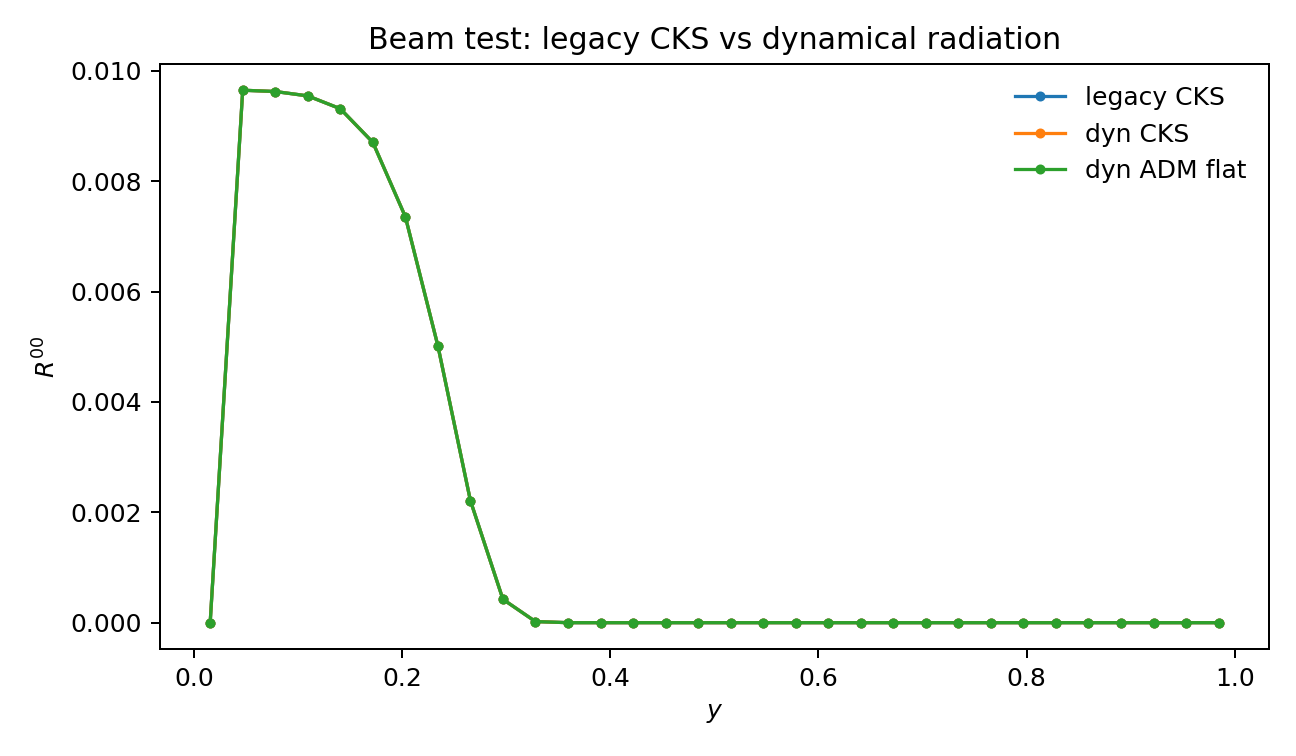
\includegraphics[width=0.82\linewidth]{figures/beam_comparison.png}
\caption{Radiation moment \(R^{00}\) along the output slice for the legacy CKS
solver, the standalone CKS-compatible branch, and the ADM flat-space branch.
The plotted profiles overlap in the current regression.}
\label{fig:beam}
\end{figure}

\begin{figure}[htbp]
\centering
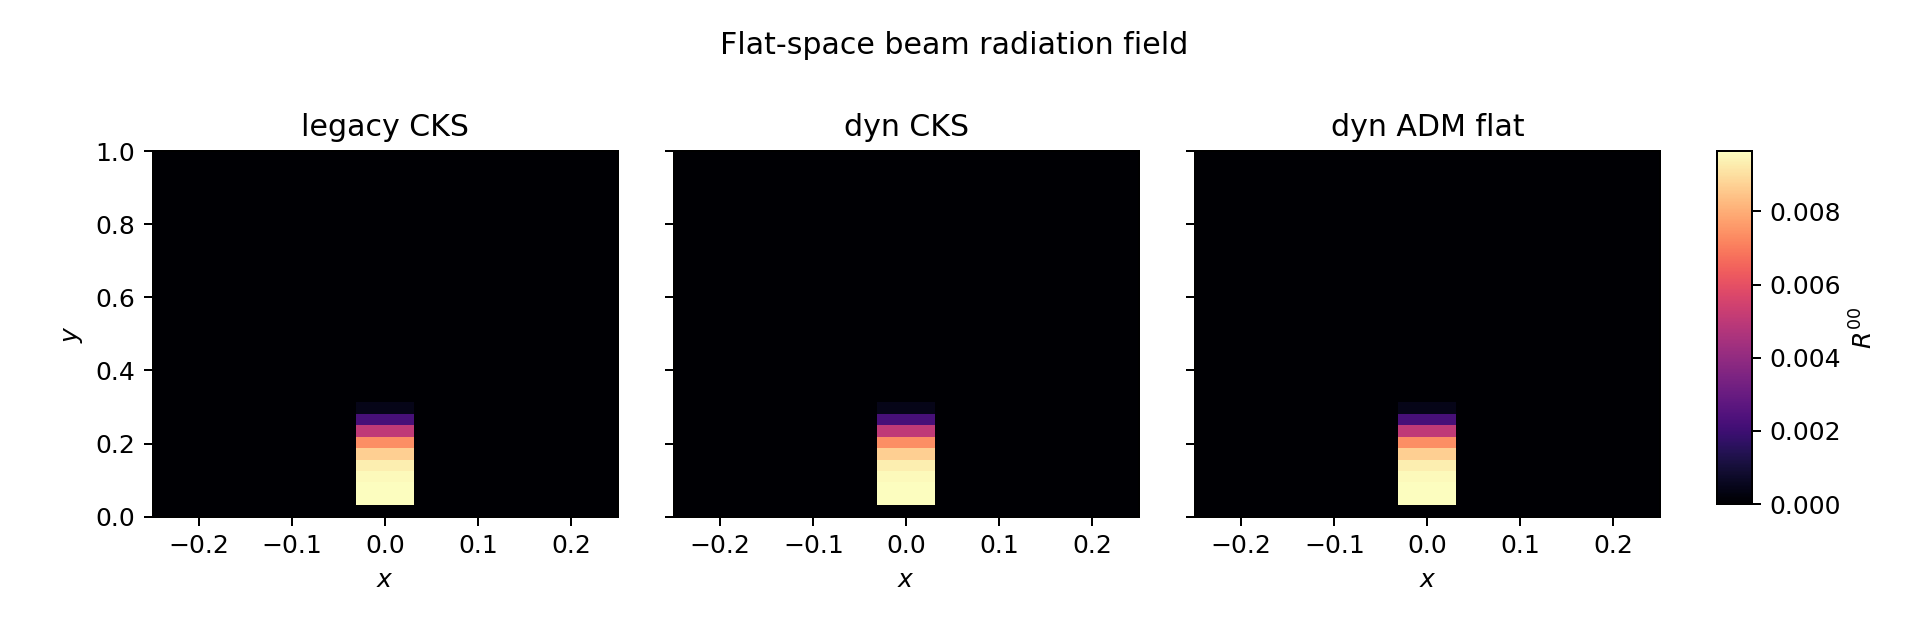
\includegraphics[width=0.95\linewidth]{figures/beam_2d_fields.png}
\caption{Two-dimensional \(R^{00}\) fields for the flat-space beam test.  The
legacy CKS solver, the standalone CKS-compatible branch, and the ADM flat-space
branch use the same color scale.}
\label{fig:beam2d}
\end{figure}

\begin{figure}[htbp]
\centering
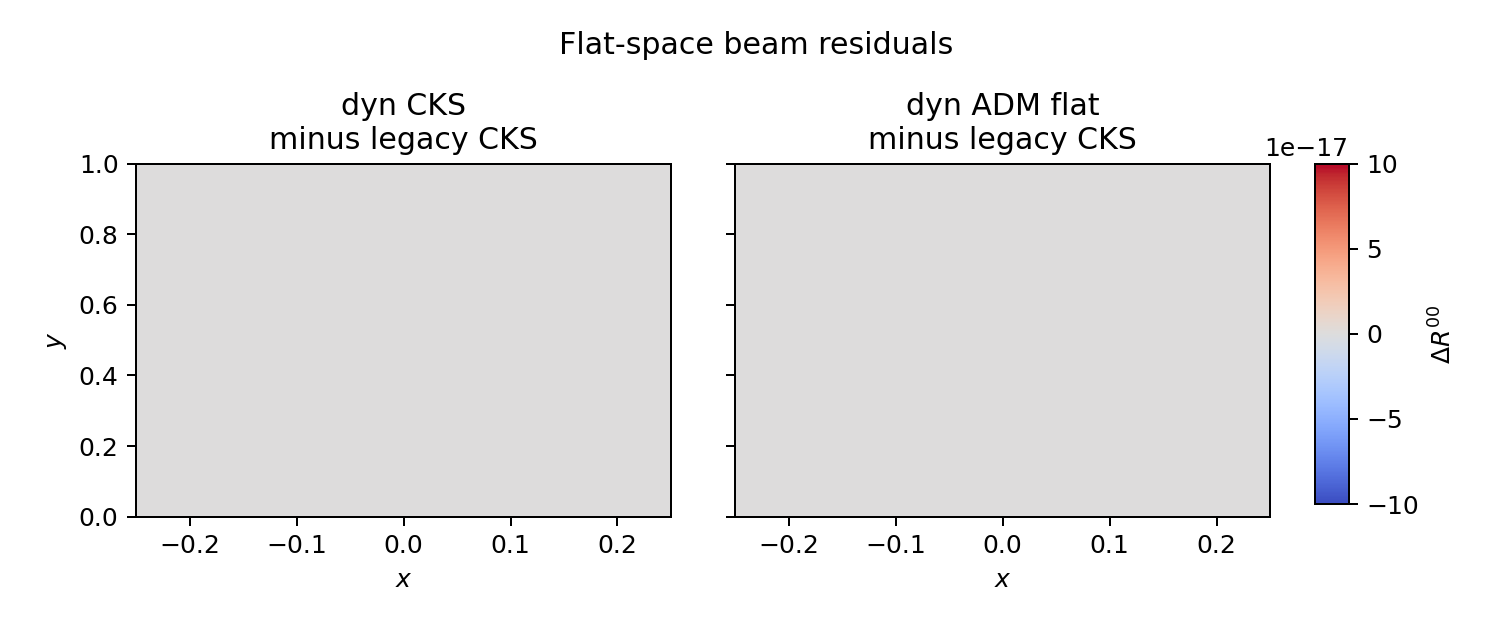
\includegraphics[width=0.86\linewidth]{figures/beam_2d_residuals.png}
\caption{Two-dimensional residuals in \(R^{00}\) for the flat-space beam test,
computed against the legacy CKS solution.  The residuals are zero to the
reported precision in the current regression.}
\label{fig:beam2dresid}
\end{figure}

\subsection{Crossing beams}

The crossing-beams regression initializes two Gaussian beams entering from the
left side of a flat domain and crossing near its center.  Because each angular
bin is transported independently, the beams should free-stream through one
another.  The built-in problem generator
\code{rad\_crossing\_beams} supports both the legacy \code{radiation} solver
and \code{dyn\_radiation}; the committed inputs are
\path{inputs/tests/rad_crossing_beams.athinput} and
\path{inputs/tests/dynrad_crossing_beams.athinput}, plus the analytic ADM
variant \path{inputs/tests/dynrad_crossing_beams_adm.athinput}.  The ADM input
uses \code{<adm dynamic=false>} with the Minkowski metric and does not enable
Z4c.  The helper script
\path{dyngr_radiation_paper/scripts/run_crossing_beams.py} runs the legacy CKS,
\code{dyn\_radiation} CKS, and \code{dyn\_radiation} ADM branches for
\(\code{nlevel}=1,\ldots,6\), plots \(R^{tt}\), and compares against the
analytic straight-line Gaussian-beam solution.

For a given angular mesh, the initialized one-sided Gaussian beam profiles start
at the marked source circles, follow the requested physical beam axes, and are
kept consistent in ghost zones by the user boundary fill.  The angular
intensities are distributed over all angular bins by a positive
maximum-entropy projection.  The projection has exact unit zeroth moment and
exact first moment along the requested beam axis at the largest realizable
positive flux factor of the finite angular grid, multiplied by the default
safety factor \(0.995\).  This avoids nearest-angle launch bias while keeping
all primitive intensities nonnegative.  The numerical and exact maps therefore
converge as angular resolution improves.  In the current run the legacy solver
and the CKS-compatible \code{dyn\_radiation} solver agree to the reported
precision for every angular resolution.  The analytic ADM branch overlays the
CKS branch visually; its normalized \(L_\infty\) difference from the CKS branch
is \(3.757567\times10^{-4}\) at \(N_{\rm ang}=12\) and
\(2.443248\times10^{-5}\) at \(N_{\rm ang}=362\).  The relative \(L_1\) error
against the analytic \(R^{tt}\) field decreases from
\(1.956930\times10^{-2}\) at \(N_{\rm ang}=12\) to
\(1.504625\times10^{-2}\) at \(N_{\rm ang}=362\) for CKS, and from
\(1.956859\times10^{-2}\) to \(1.504618\times10^{-2}\) for ADM.  The remaining
error is set by the finite angular direction set and spatial advection
diffusion.

\begin{figure}[htbp]
\centering
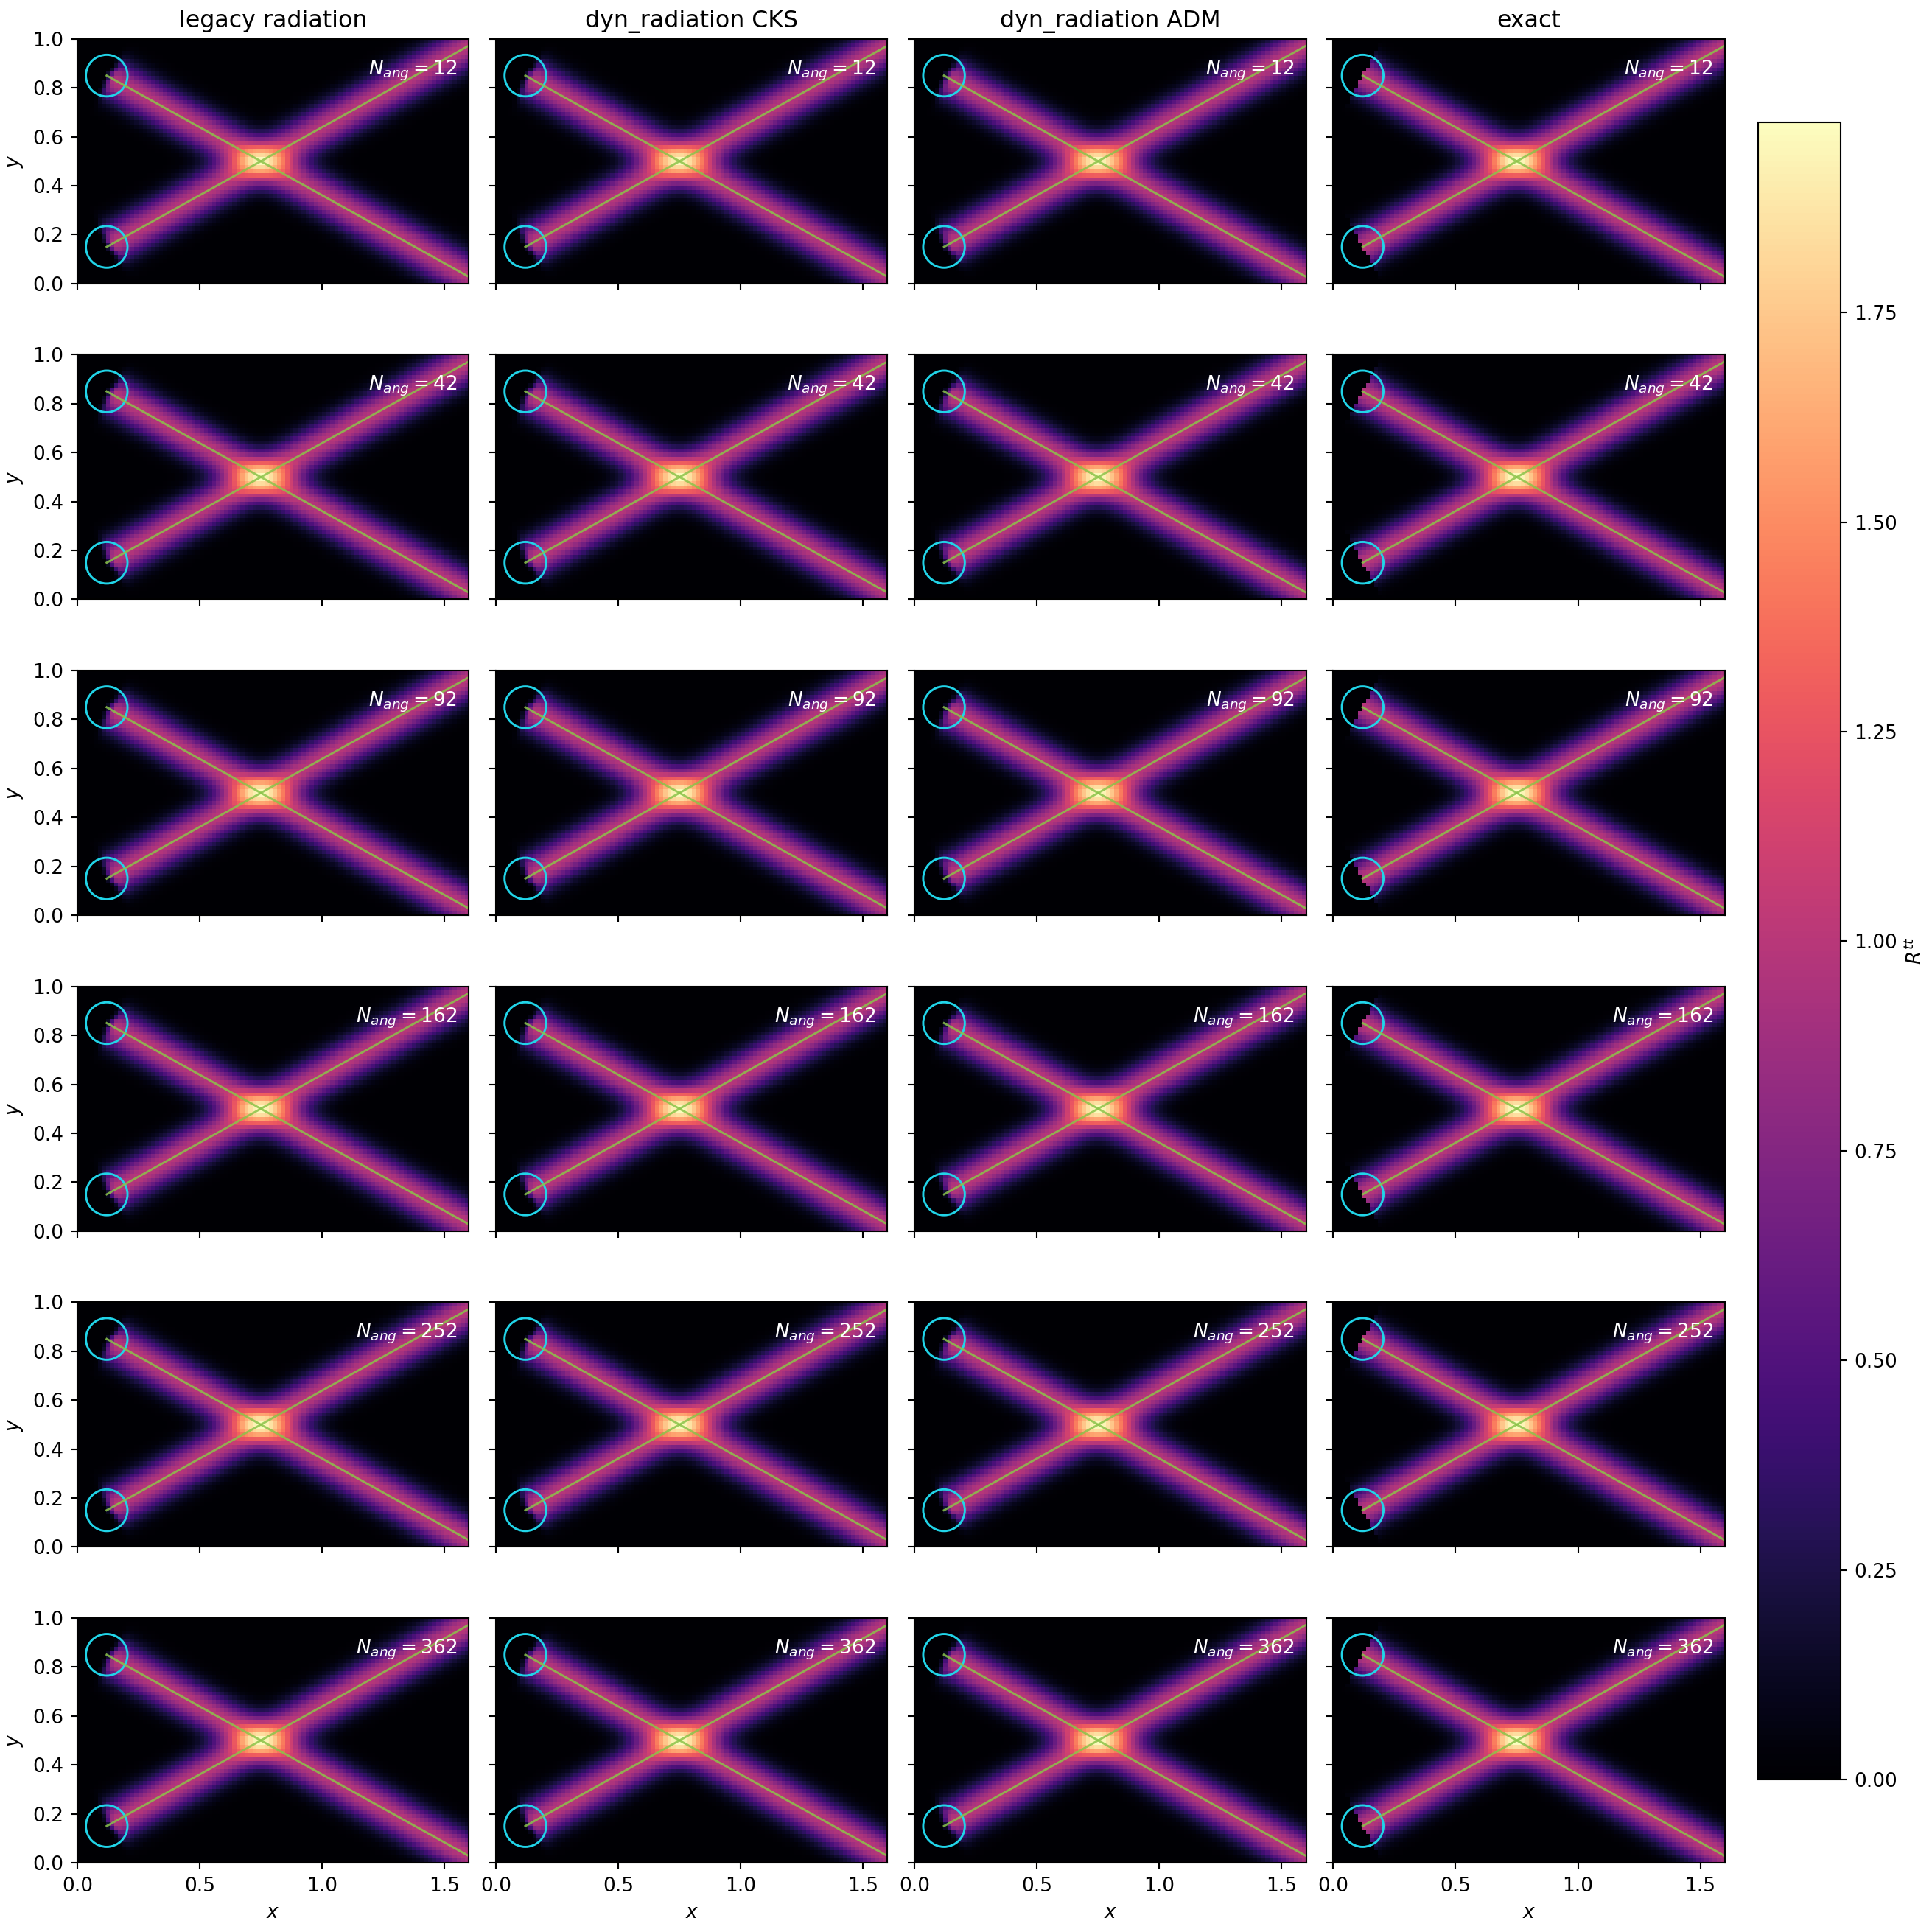
\includegraphics[width=0.98\linewidth]{figures/crossing_beams_comparison.png}
\caption{Crossing-beams \(R^{tt}\) maps for the legacy solver,
\code{dyn\_radiation} in CKS compatibility mode, \code{dyn\_radiation} with
analytic Minkowski ADM data, and the analytic solution.  The numerical columns
overlap in the current regression and approach the analytic beam geometry as
\(N_{\rm ang}\) increases.}
\label{fig:crossingbeams}
\end{figure}

\begin{figure}[htbp]
\centering
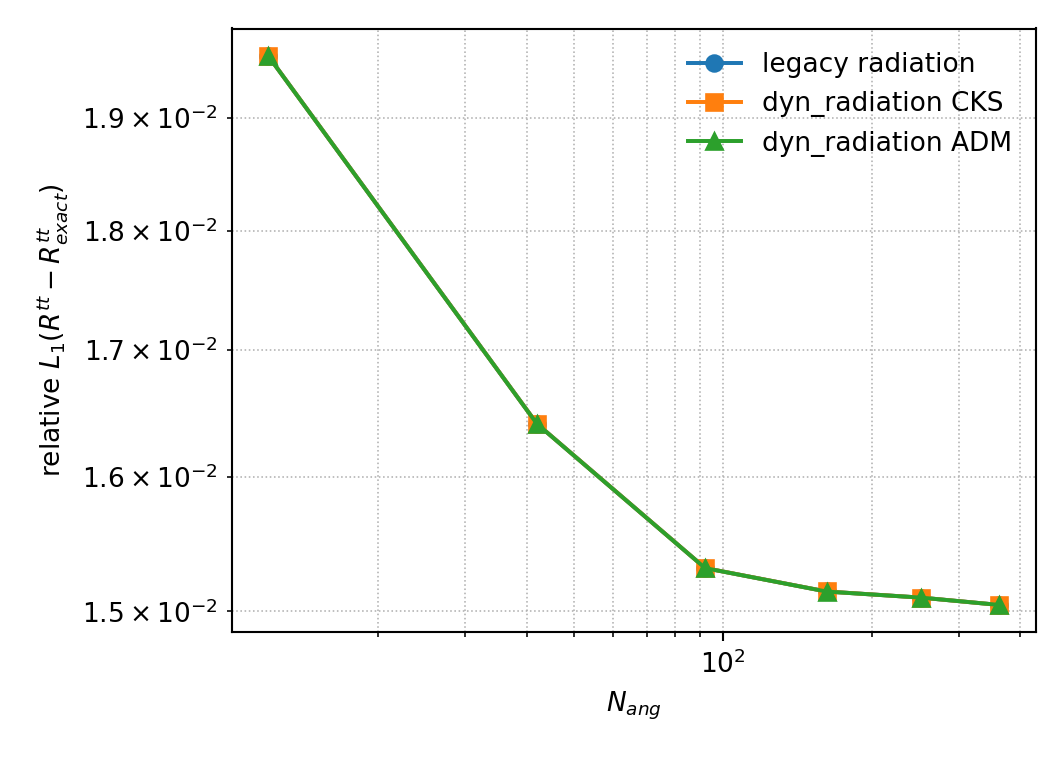
\includegraphics[width=0.62\linewidth]{figures/crossing_beams_convergence.png}
\caption{Relative \(L_1\) error of the crossing-beams \(R^{tt}\) field against
the analytic straight-line Gaussian-beam solution as the angular mesh is
refined.}
\label{fig:crossingbeamsconv}
\end{figure}

\subsection{Kerr photon-orbit beam}

The black-hole beam regression uses the same stationary Kerr-Schild geometry in
the legacy solver, the CKS-compatible \code{dyn\_radiation} branch, and the
analytic ADM \code{dyn\_radiation} branch.  The ADM input uses
\code{<adm dynamic=false>} with the Kerr-Schild metric and does not enable Z4c.
The built-in problem generator \code{rad\_kerr\_orbit\_beam} enrolls a user
radiation source term rather than the legacy cone source.  At setup it computes
the equatorial counter-rotating Kerr photon-orbit radius for the requested spin,
maps the tangent null direction into the local tetrad at the source, and
projects that direction onto a positive angular stencil.  The source then adds
intensity with unit angular zeroth moment and first moment parallel to the
photon-orbit tangent.  This avoids a nearest-angle launch error while retaining
a compact local setup with \(n_{x_3}=1\).

The committed inputs are
\path{inputs/tests/rad_kerr_orbit_beam.athinput} and
\path{inputs/tests/dynrad_kerr_orbit_beam.athinput}, plus the ADM variant
\path{inputs/tests/dynrad_kerr_orbit_beam_adm.athinput}.  The helper script
\path{dyngr_radiation_paper/scripts/run_kerr_orbit_beam.py} runs all three
branches and overlays the analytic equatorial photon-orbit guide.  With
\(\code{nlevel}=4\) (\(N_{\rm ang}=162\)) and a \(72\times72\times1\) mesh, the
normalized infinity-norm difference between the CKS \code{dyn\_radiation} map
and the legacy CKS map is \(7.298162\times10^{-2}\) after \(t=5\), with a
relative \(L_1\) difference of \(1.595626\times10^{-2}\).  The ADM map follows
the same photon-orbit guide; its normalized infinity-norm difference from the
CKS \code{dyn\_radiation} map is \(4.497598\times10^{-2}\), with a relative
\(L_1\) difference of \(7.477185\times10^{-2}\).  The largest discrepancies
occur along weak, angularly diffused beam shoulders; the high-intensity ridge
follows the same guide in all three branches.

\begin{figure}[htbp]
\centering
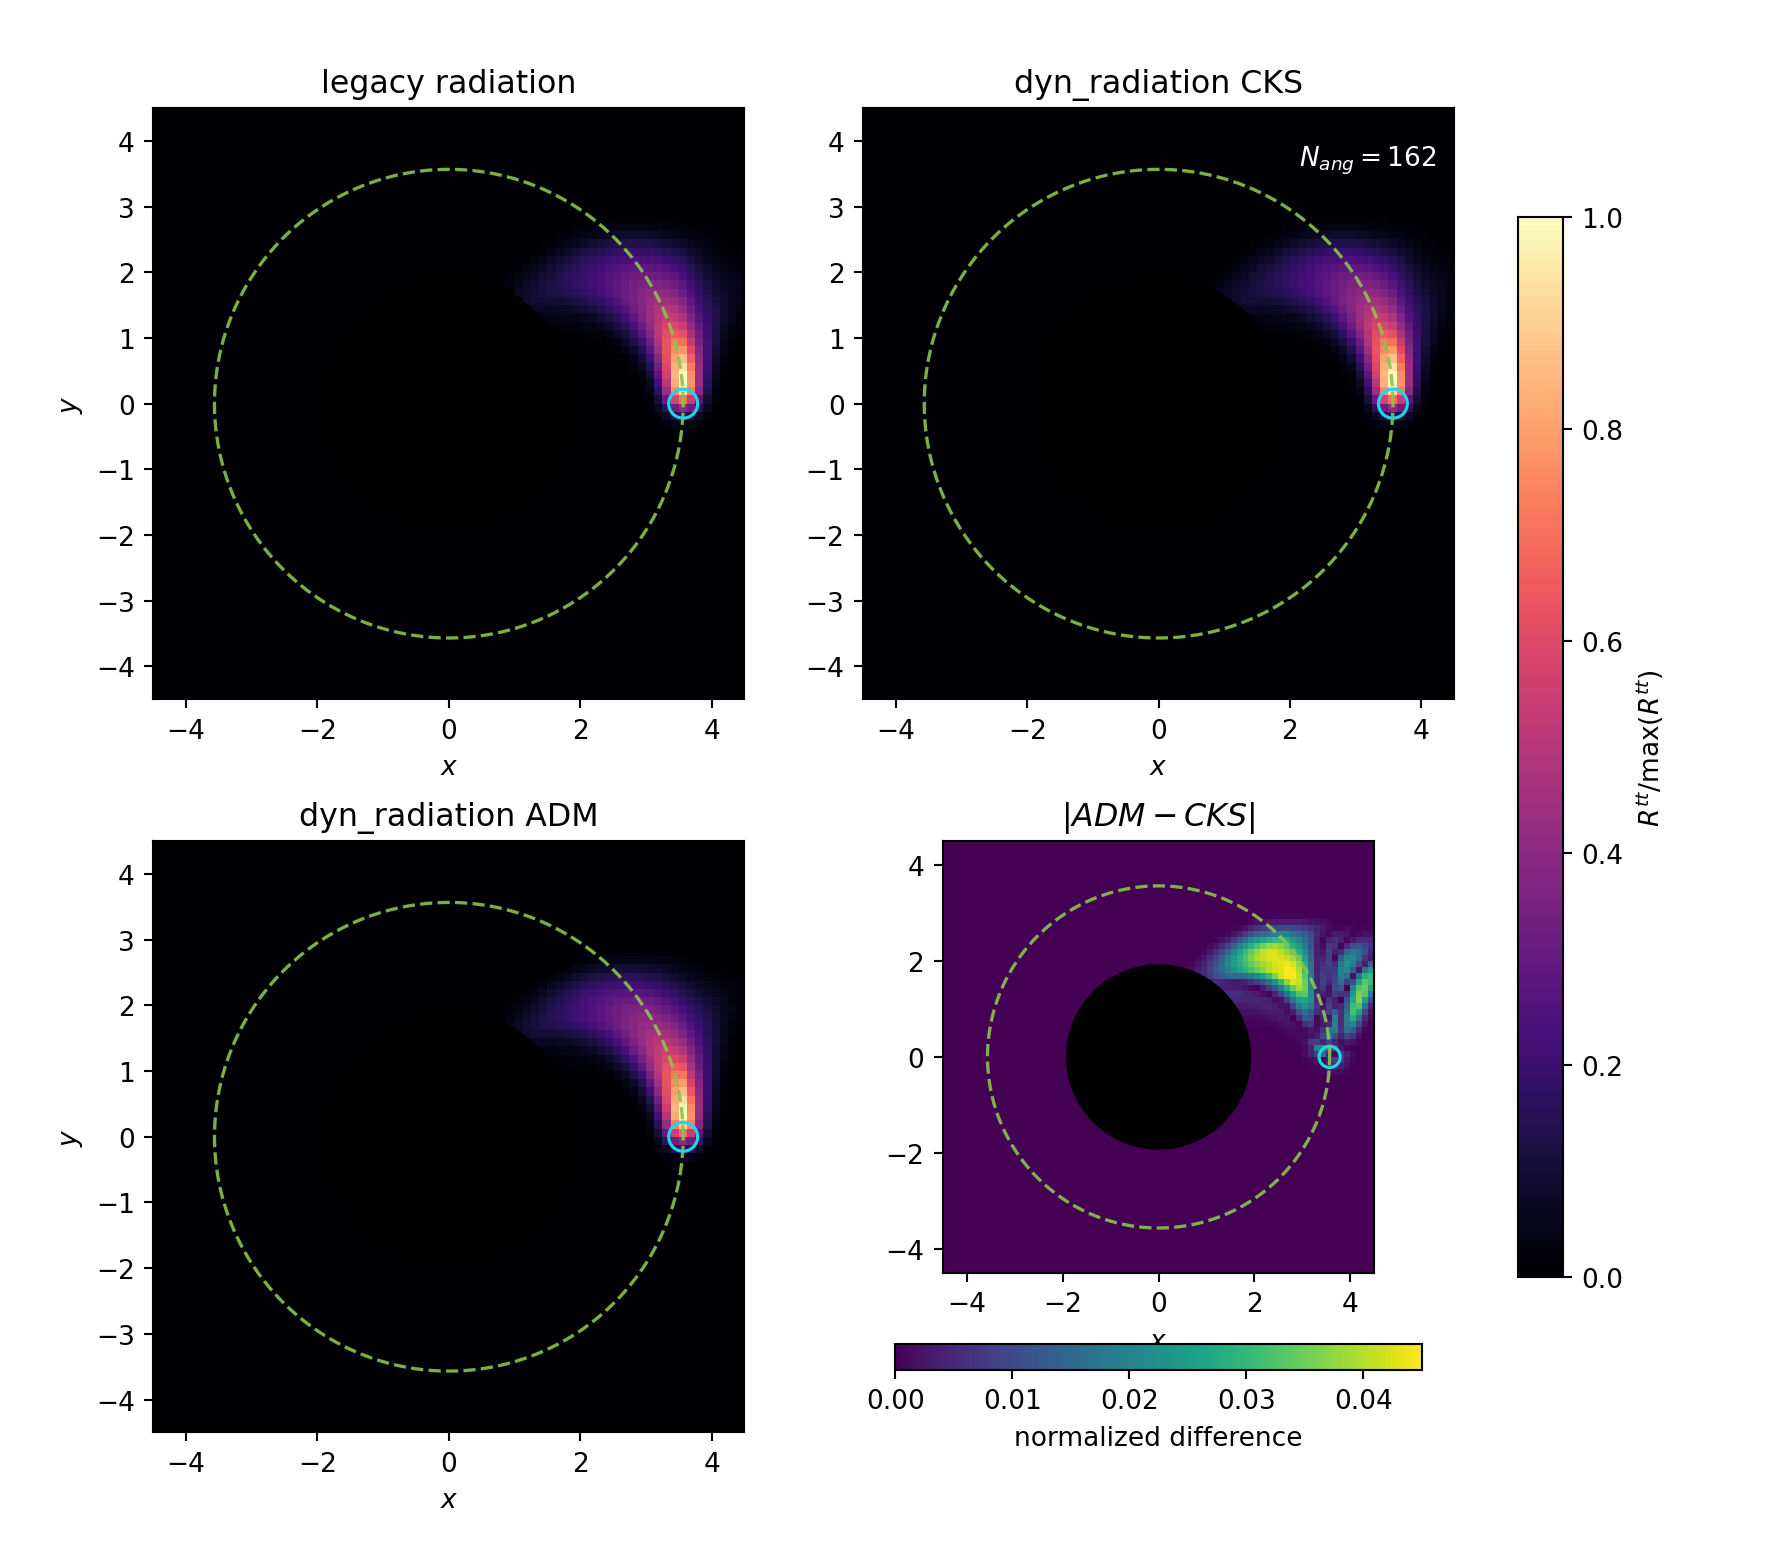
\includegraphics[width=0.98\linewidth]{figures/kerr_orbit_beam_comparison.png}
\caption{Kerr photon-orbit beam comparison.  The dashed green curve is the
equatorial photon-orbit guide, the cyan circle marks the projected source
region, and the black disk marks the horizon-scale excision region.  The panels
compare the legacy CKS solver, \code{dyn\_radiation} CKS, analytic ADM
\code{dyn\_radiation}, and the normalized ADM-CKS difference on the same compact
\(n_{x_3}=1\) grid.}
\label{fig:kerrbeam}
\end{figure}

\subsection{Gas-radiation equilibration}

The homogeneous equilibration regression initializes gas and radiation out of
thermal equilibrium and evolves only the local absorption/emission source.
The built-in problem generator \code{rad\_equilibration} supports both
\code{radiation} and \code{dyn\_radiation}; the paired inputs are
\path{inputs/tests/rad_equilibration.athinput} and
\path{inputs/tests/dynrad_equilibration.athinput}.  The default setup uses
\(\rho=1\), \(\Gamma=5/3\), \(T_{\rm gas}(0)=2\),
\(T_{\rm rad}(0)=1\), \(a_{\rm rad}=1\), pure absorption
\(\kappa_a=1\), and a homogeneous periodic mesh.  With
\(c_V=\rho/(\Gamma-1)\), the conserved total energy density is
\[
  u_{\rm tot}=c_V T_{\rm gas}+a_{\rm rad}T_{\rm rad}^4=4.
\]
The exact comparison curve solves the scalar ODE
\[
  c_V\frac{dT_{\rm gas}}{d\tau}
    =-\left(a_{\rm rad}T_{\rm gas}^4
      - \left[u_{\rm tot}-c_VT_{\rm gas}\right]\right),
  \qquad
  T_{\rm rad}=\left(\frac{u_{\rm tot}-c_VT_{\rm gas}}
      {a_{\rm rad}}\right)^{1/4},
\]
where \(\tau=\kappa_a t\).  The script
\path{dyngr_radiation_paper/scripts/run_equilibration.py} runs both solvers
with effective 1-step, 10-step, and 100-step source integrations to
\(\tau=1\), overlays the exact ODE solution, and checks conservation of
\(u_{\rm tot}\).  In the current run the 100-step \code{dyn\_radiation}
solution had maximum errors
\(\max|\Delta T|=1.712653\times10^{-2}\) and
\(\max|\Delta u|=2.568980\times10^{-2}\) against the exact curve.  The final
states of the legacy and \code{dyn\_radiation} runs agreed:
\(T_{\rm gas}=1.216323\), \(T_{\rm rad}=1.214481\), and
\(u_{\rm tot}=4.000000\).

\begin{figure}[htbp]
\centering
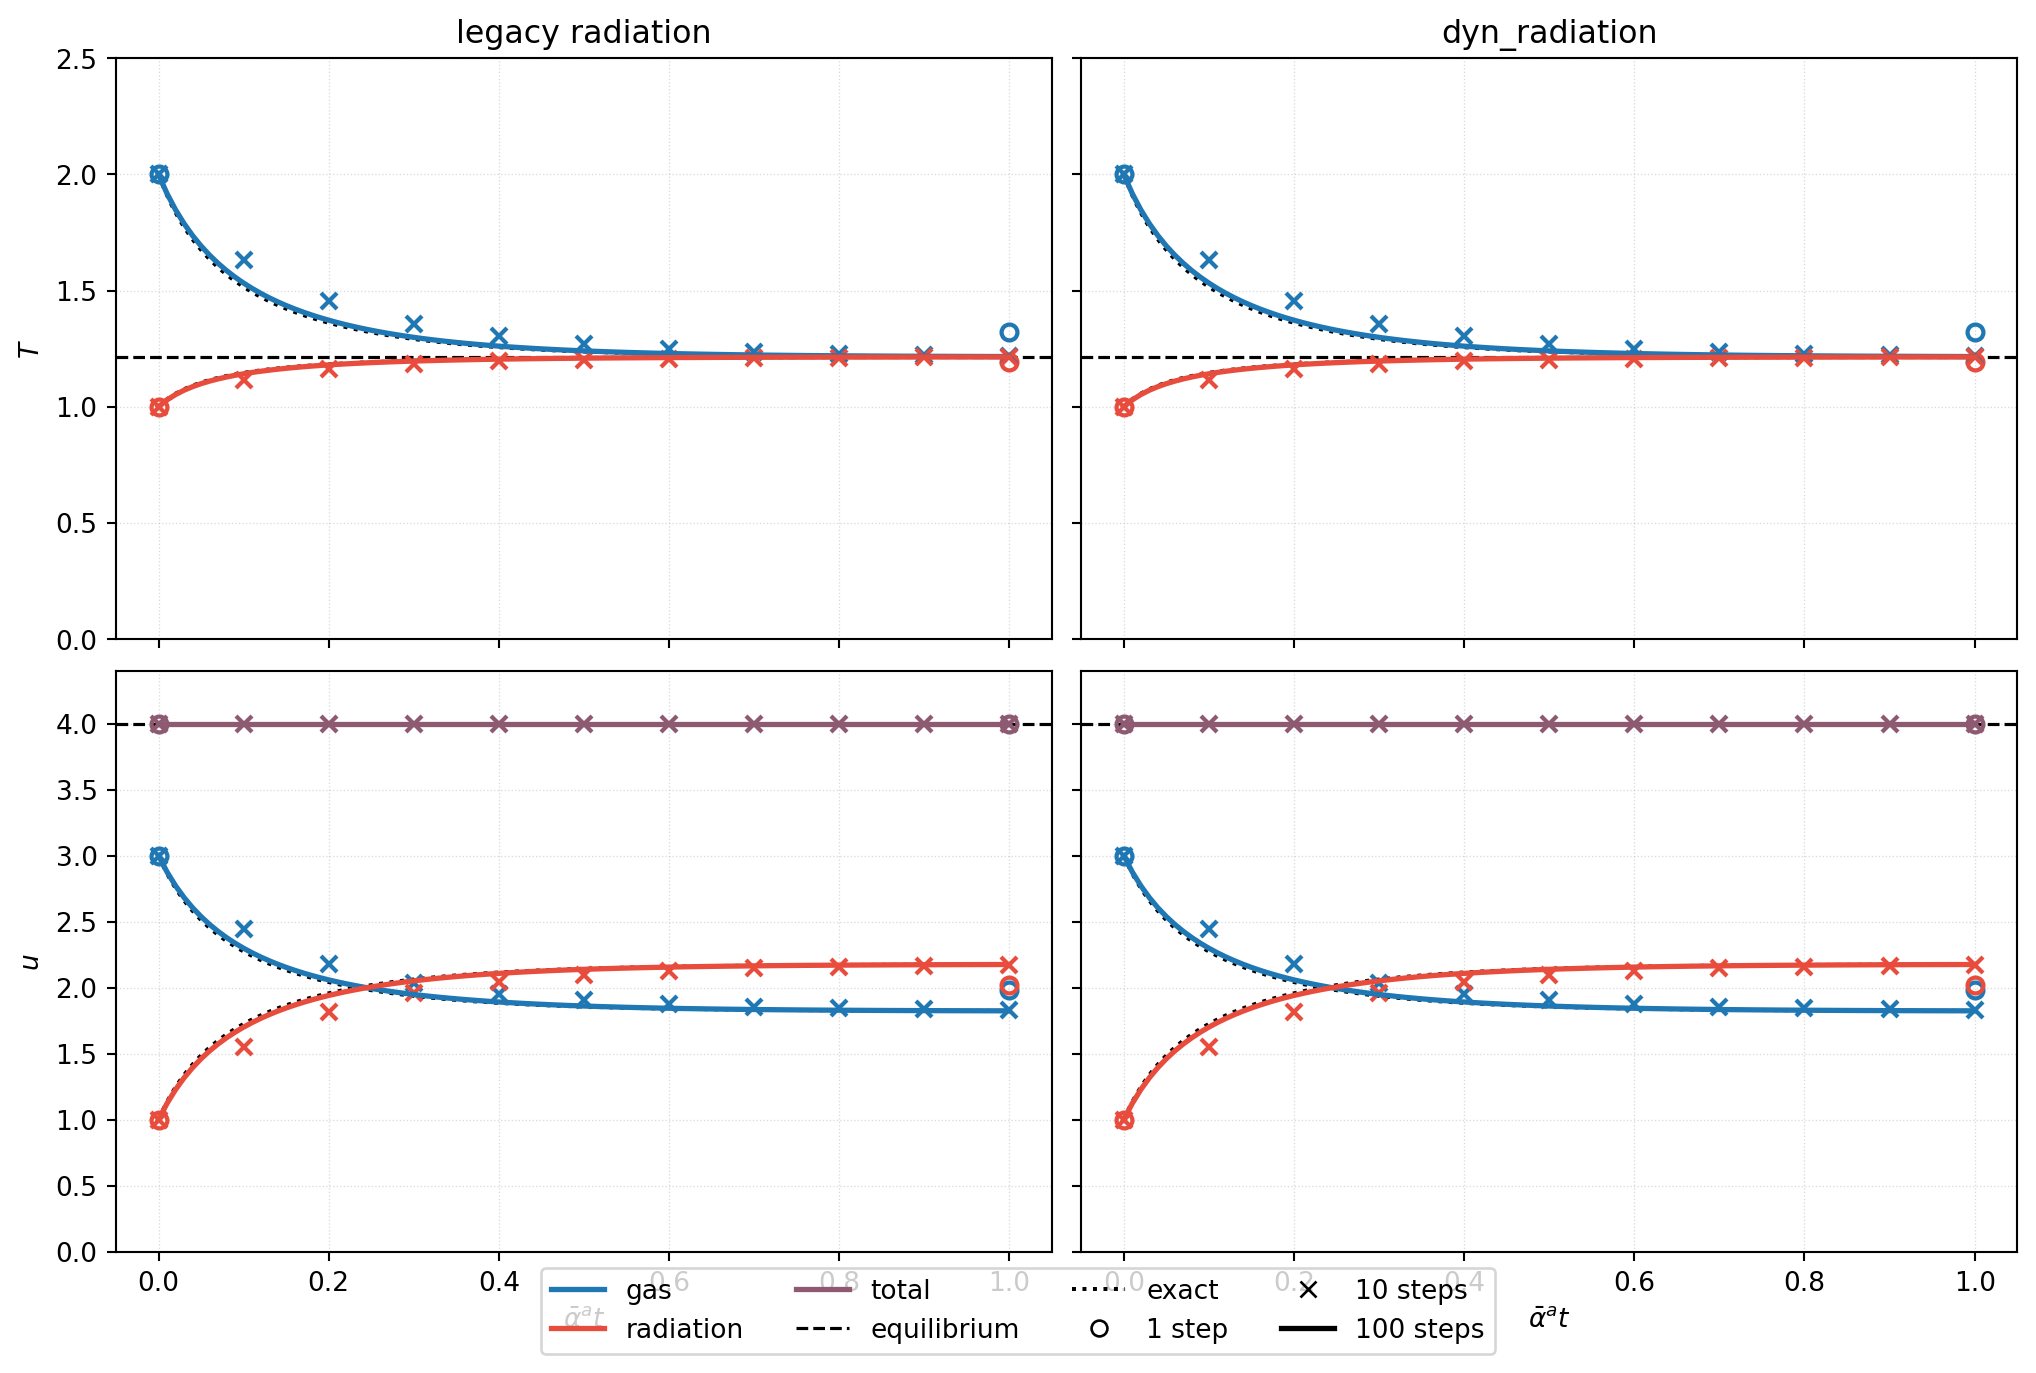
\includegraphics[width=0.98\linewidth]{figures/equilibration_comparison.png}
\caption{Homogeneous gas-radiation equilibration for the legacy solver and
\code{dyn\_radiation}.  Symbols show coarse source-step integrations, solid
curves show the 100-step run, dashed lines mark the equilibrium state, and
dotted curves show the exact energy-conserving relaxation ODE.}
\label{fig:equilibration}
\end{figure}

\subsection{Radiation-hydrodynamic linear wave}

The stationary CKS compatibility branch was also checked against the legacy
radiation solver on a radiation-hydrodynamic linear wave.  The final error rows
match:
\begin{equation}
\begin{split}
  \mathrm{RMS}\mbox{-}L_1 &= 2.400907\times10^{-6},\\
  d_{L_1} &= 1.685676\times10^{-6},\\
  M^1_{L_1} &= 1.380892\times10^{-6},\\
  E_{L_1} &= 1.007962\times10^{-6}.
\end{split}
\end{equation}
The corresponding inputs are
\path{dyngr_radiation_paper/inputs/lwave_radiation_cks.athinput} and
\path{dyngr_radiation_paper/inputs/lwave_dynrad_cks.athinput}.

\begin{figure}[htbp]
\centering
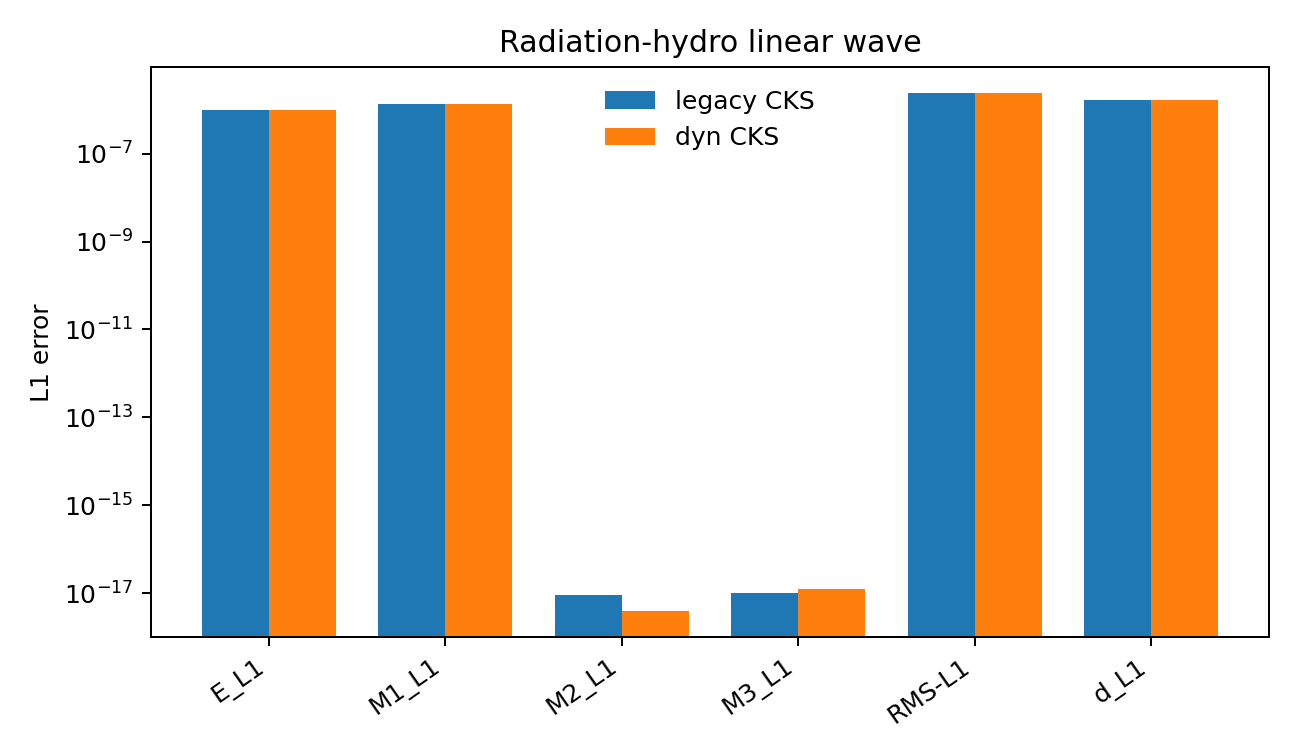
\includegraphics[width=0.82\linewidth]{figures/linear_wave_errors.png}
\caption{Linear-wave error metrics for the legacy solver and
\code{dyn\_radiation} in stationary CKS compatibility mode.}
\label{fig:lwave}
\end{figure}

The convergence form of the same test is generated by
\path{dyngr_radiation_paper/scripts/run_linear_wave_convergence.py} from
\path{inputs/tests/rad_lwave_convergence.athinput},
\path{inputs/tests/dynrad_lwave_convergence.athinput}, and
\path{inputs/tests/dynrad_lwave_adm_convergence.athinput}.  The ADM input uses
\code{<adm dynamic=false>} with the analytic Minkowski ADM metric and a
zero-field \code{<mhd>} wrapper, because ADM/Z4c backgrounds are connected to
the fluid package through dynGRMHD rather than \code{<hydro>}.  These runs use
\(\delta=10^{-4}\), which is small enough to remain in the linear regime but
large enough that the final binary outputs are not limited by single-precision
output quantization.  The script measures normalized \(L_1\) errors in
\(\rho\), \(u^x\), \(P_{\rm gas}\), \(R^{tt}\), and \(R^{tx}\) directly
against the analytic eigenmode at \(N_{\rm cell}=16,32,64,128,256\).  The
legacy, CKS \code{dyn\_radiation}, and analytic-flat ADM
\code{dyn\_radiation} curves overlap to plotting precision.  The
last-three-point convergence rates in the current run were
\[
\begin{array}{c|cccccc}
 & {\rm RMS} & \rho & u^x & P_{\rm gas} & R^{tt} & R^{tx} \\
\hline
{\rm dyn\ CKS} & 2.071 & 1.849 & 2.129 & 2.111 & 2.121 & 2.247 \\
{\rm dyn\ ADM} & 2.070 & 1.849 & 2.129 & 2.105 & 2.121 & 2.247
\end{array}
\]
which is consistent with the second-order reconstruction and RK2 time
integration used in the input.  The density rate is slightly lower over this
finite range because that component is closest to the binary-output precision
floor at the highest resolution.

\begin{figure}[htbp]
\centering
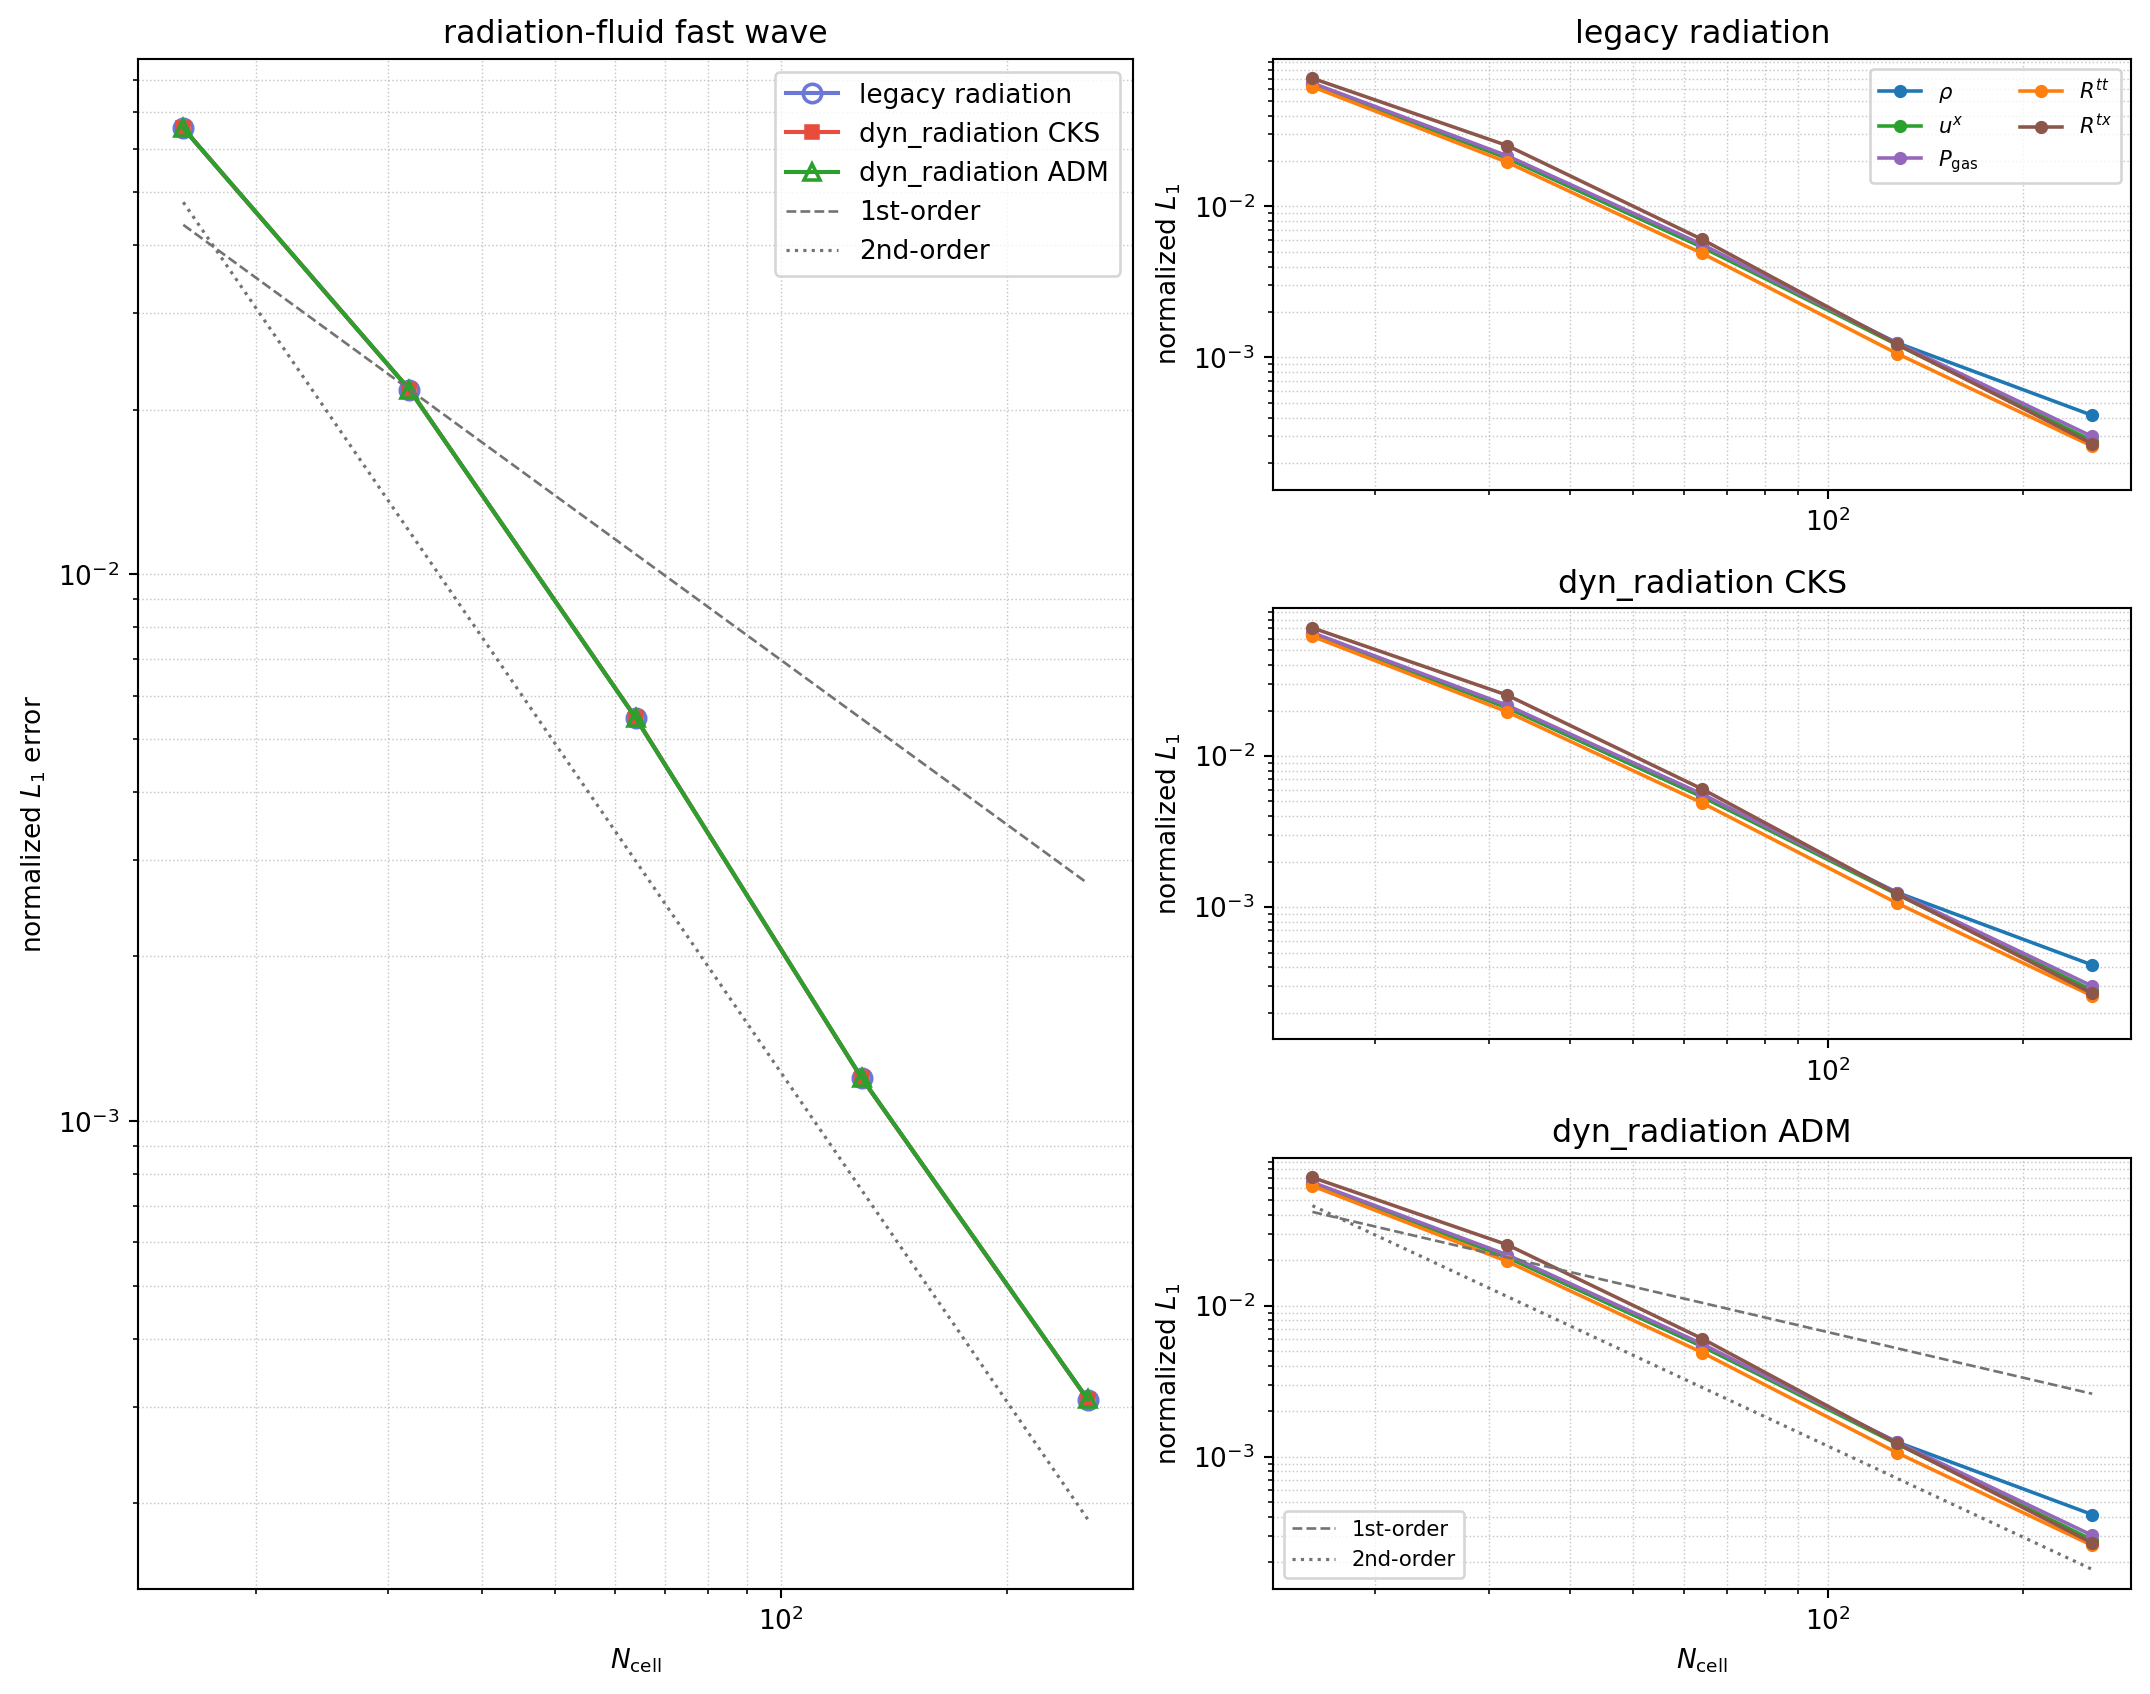
\includegraphics[width=0.98\linewidth]{figures/linear_wave_convergence.png}
\caption{Radiation-fluid linear-wave convergence.  The left panel shows
the normalized coupled \(L_1\) error for the legacy CKS solver,
\code{dyn\_radiation} in CKS mode, and \code{dyn\_radiation} in analytic-flat
ADM mode; the curves overlap.  The right panels split the error by fluid and
radiation-moment components for each solver path.}
\label{fig:lwaveconv}
\end{figure}

\subsection{ADM formal regressions}

Three additional compact regressions target the ADM-only pieces that are not
isolated by the flat CKS compatibility tests.  The committed inputs are
\path{inputs/tests/dynrad_flrw_redshift.athinput},
\path{inputs/tests/dynrad_lapse_gradient.athinput}, and
\path{inputs/tests/dynrad_momentum_source.athinput}; the helper script
\path{dyngr_radiation_paper/scripts/run_adm_formal_tests.py} reruns them and
writes Figure~\ref{fig:admformal}.  These tests use \code{<adm dynamic=false>}
with analytic ADM data supplied by the problem generator, so they exercise the
ADM radiation geometry path without invoking Z4c.

The FLRW redshift test sets
\(\alpha=1\), \(\beta^i=0\),
\(\gamma_{ij}=a(t)^2\delta_{ij}\), and
\(K_{ij}=-a\dot a\,\delta_{ij}\), with \(a(t)=1+0.2t\).  A homogeneous
isotropic radiation field should satisfy \(E\propto a^{-4}\) and
\(\sqrt{\gamma}E\propto a^{-1}\).  The current run to \(t=0.5\) gave
\(E=0.6829324379755602\) against \(a^{-4}=0.6830134553650705\), and
\(\sqrt{\gamma}E=0.908983074945471\) against \(a^{-1}=0.9090909090909091\);
both relative errors were \(1.18618\times10^{-4}\).  This checks the sign of
\(\alpha K_{ij}s^is^j\) in the geometric energy source.

The static lapse-gradient test sets
\(\alpha(x)=1+0.1\sin(2\pi x)\), \(\beta^i=0\), and
\(\gamma_{ij}=\delta_{ij}\), and initializes a uniform anisotropic radiation
field with positive \(x\)-directed flux.  For the short run
\(t=0.01\), the first-order source prediction is
\(\Delta E=-2E_0 f_x(\partial_x\alpha)t\).  The numerical perturbation has
correlation \(0.999307\) with that analytic shape and relative RMS mismatch
\(4.68375\times10^{-2}\), consistent with using the full transport update
rather than an isolated infinitesimal source step.

The momentum-source closure test compares the angular sum of the ADM
Hamiltonian force,
\(\sum_n w_n I_n A_j\), to the Valencia momentum source
\[
  -E\,\partial_j\alpha
  + S_i\,\partial_j\beta^i
  + \frac{1}{2}\alpha P^{ik}\partial_j\gamma_{ik}.
\]
The two sides are evaluated from the same cached ADM gradients used by the
solver.  The maximum absolute mismatch decreased from
\(1.80196\times10^{-5}\) at \(N_x=32\) to
\(1.14669\times10^{-6}\) at \(N_x=128\), following the expected second-order
finite-difference cache error.  The maximum relative mismatch at \(N_x=128\)
was \(8.47848\times10^{-4}\); that relative norm is dominated by cells where
the source denominator is small.

\begin{figure}[htbp]
\centering
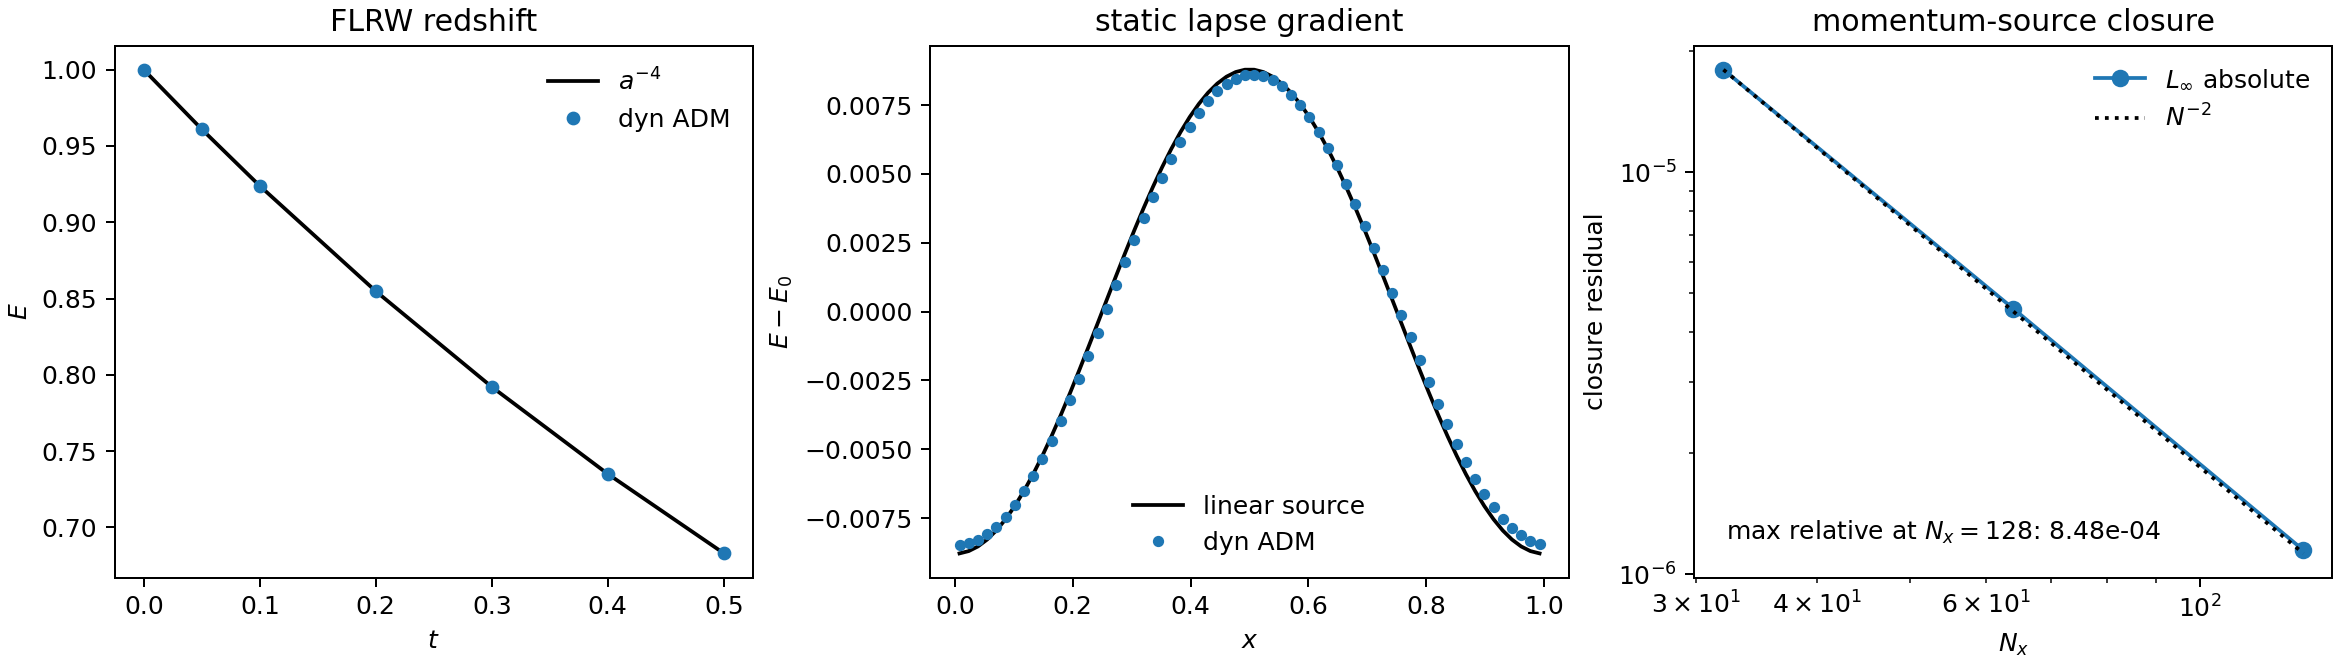
\includegraphics[width=0.98\linewidth]{figures/adm_formal_tests.png}
\caption{ADM-specific formal regressions.  Left: homogeneous FLRW radiation
redshifts as \(E\propto a^{-4}\).  Center: the static lapse-gradient source has
the predicted sign and shape.  Right: the Hamiltonian angular-force sum and the
Valencia momentum source agree with a second-order absolute residual as the
ADM metric-gradient cache is refined.}
\label{fig:admformal}
\end{figure}

\subsection{Binary-background beam and particle smoke test}

The binary-background input is
\begin{center}
\small
\path{dyngr_radiation_paper/inputs/dynbbh_beam_particles.athinput}.
\end{center}
It exercises the ADM beam source on the superposed boosted Kerr-Schild binary
background in \code{src/pgen/dynbbh.cpp}.  It runs with
\code{geometry=adm}, \code{angular\_fluxes=true}, and
\code{adm/dynamic=true}; the latter is required because the analytic
superposed-BBH ADM callback depends on \code{pmesh->time}.  The dynbbh initializer
now uses only \code{pdynrad}; the legacy \code{prad} path is rejected because
its stationary CKS normalization is inconsistent with the ADM background.  It
also initializes null
particles on the beam edge and advances them using Equations~\eqref{eq:null_x}
and \eqref{eq:null_k}.  The committed input remains a short smoke test
(\(t=0.2\)); the figure runner
\path{dyngr_radiation_paper/scripts/run_dynbbh_beam_figures.py} overrides the
same input for plotting.  The current high-resolution figure run uses a
\(72\times72\times4\) mesh, \(36\times36\times4\) MeshBlocks, \(N_{\rm ang}\)
from \code{nlevel=4}, four MPI ranks, a \(20^\circ\) source cone, and advances
to \(t=10\).  This matches the single-BH angular resolution while keeping the
minimum active \(x^3\) resolution accepted by the mesh driver.  It completed in
181 cycles with empty stderr; the final lineout has
\(\max R^{tt}=6.247600\) and lineout integral \(6.491427\).  The dynbbh pgen
drops non-source-rank placeholder particles in MPI and retags the remaining
source particles, so the tracked-particle output follows only real null beam
tracers.  The radiation source is a fixed coordinate-time, fixed
coordinate-direction injection; the dashed guide in the figures marks this
source axis rather than an expected geodesic in the curved, time-dependent
background.  The radiation maps, ADM lapse/conformal-factor background, null
beam-edge trajectories, and time-series snapshots are shown in
Figures~\ref{fig:dynbbhsummary}, \ref{fig:dynbbhtimeseries}, and
\ref{fig:dynbbhlineout}.  A separate serial run enabled ADM radiation-matter
coupling with absorption and scattering opacities and completed without NaNs.
These are compact runtime tests; long production dynbbh/MHD radiation
evolutions remain a separate validation target.

\begin{figure}[htbp]
\centering
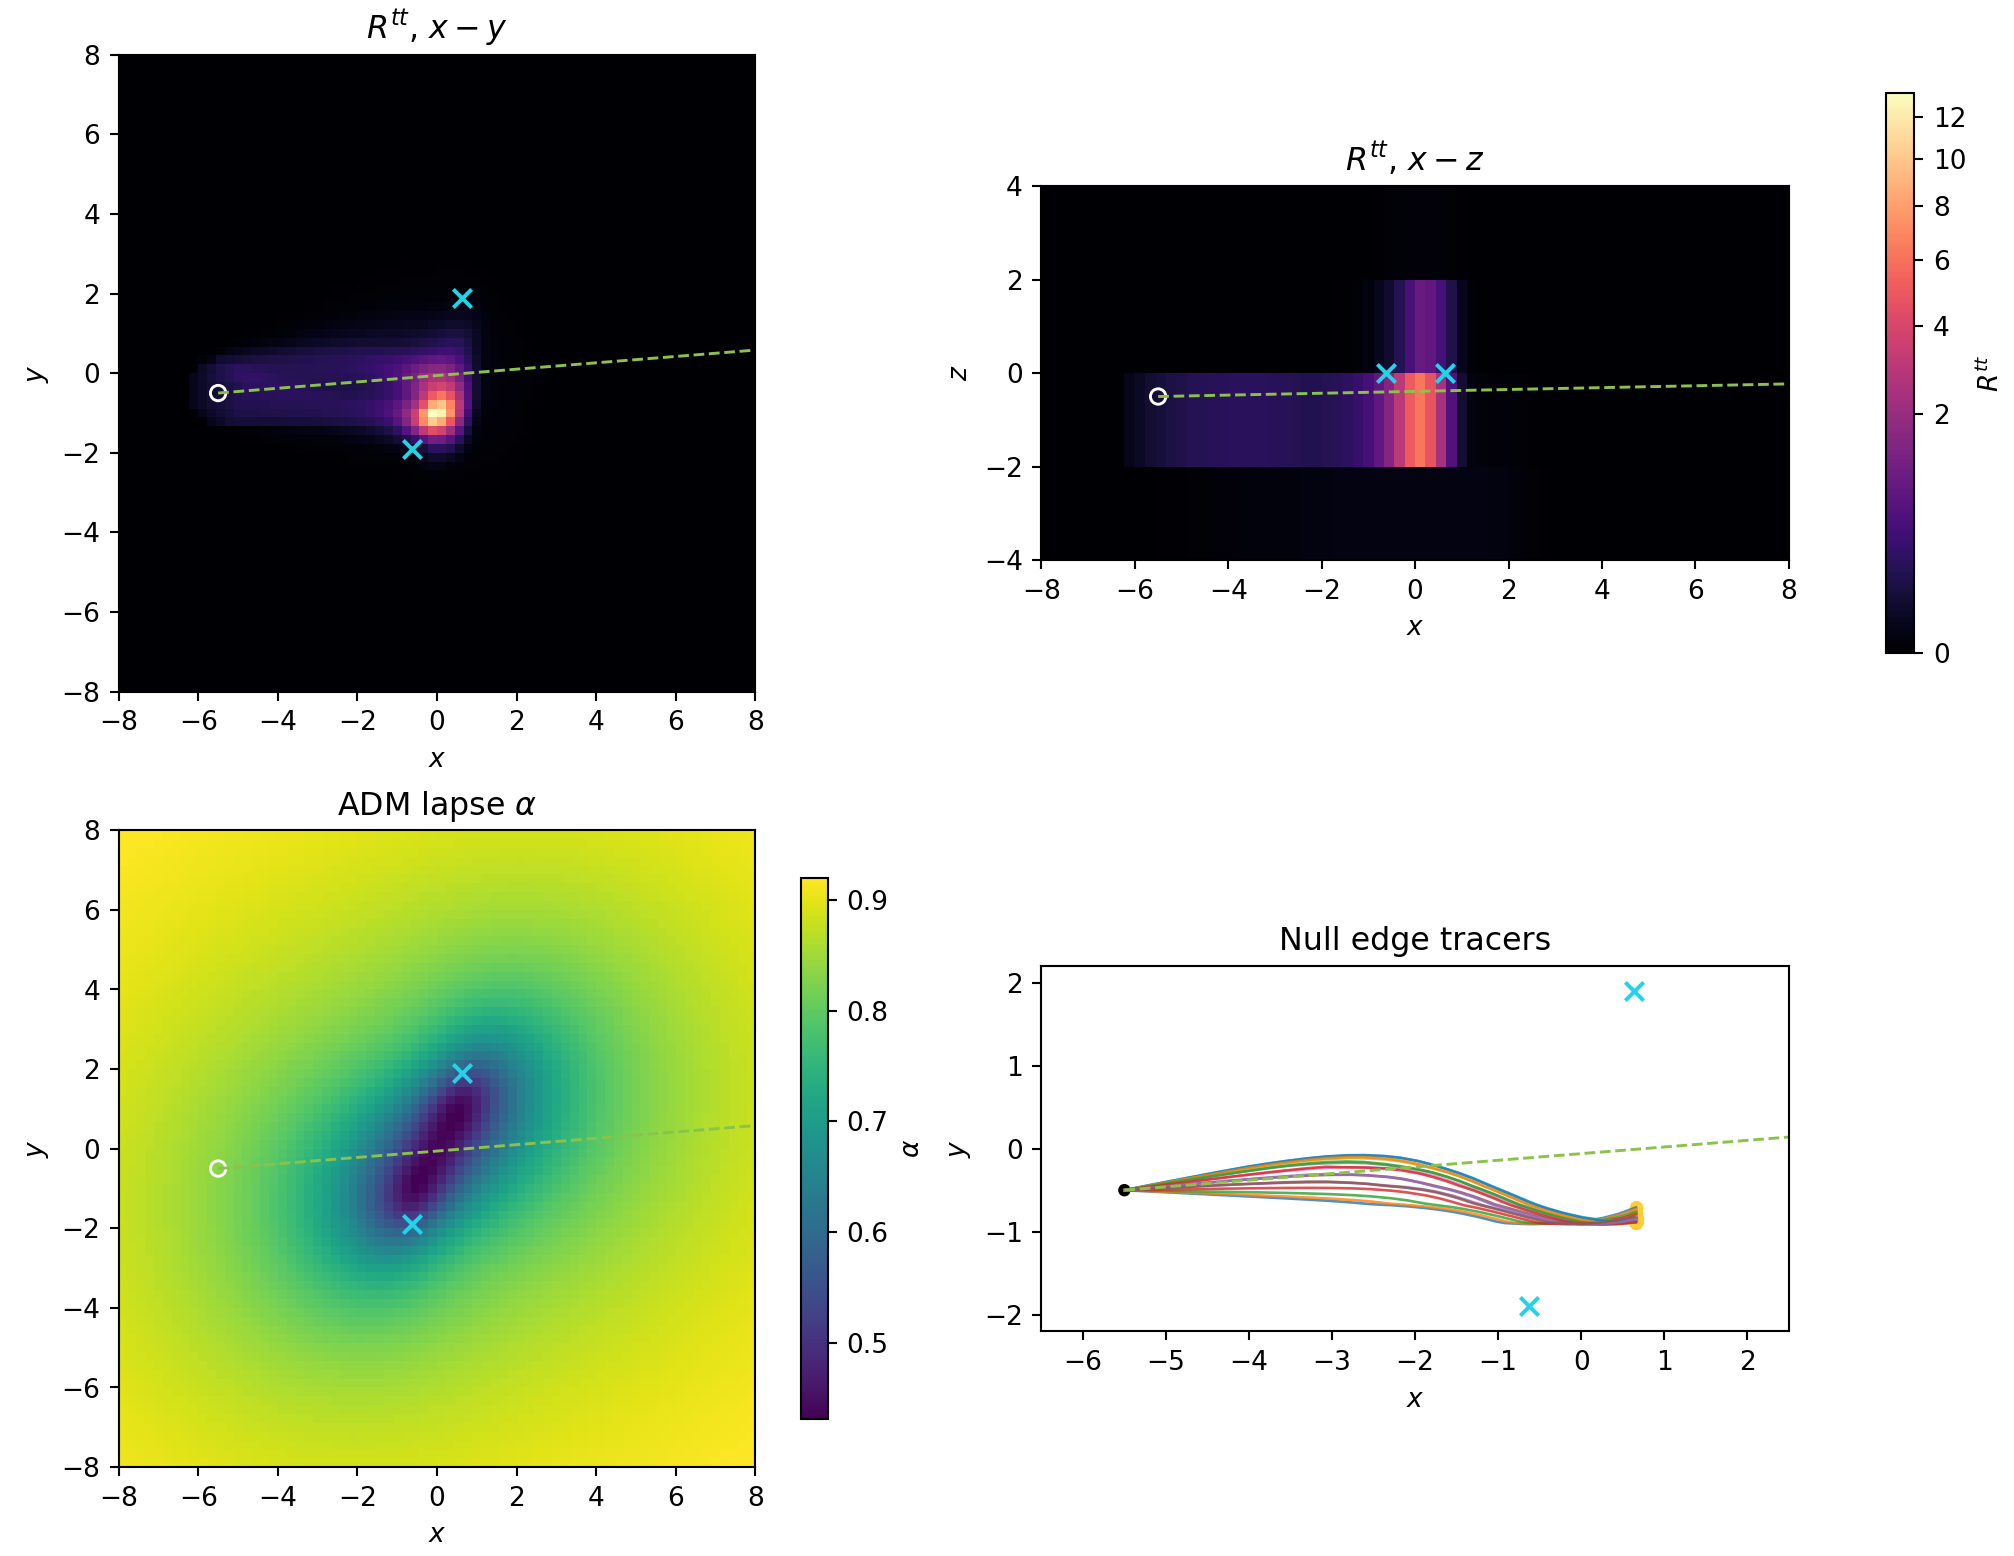
\includegraphics[width=0.98\linewidth]{figures/dynbbh_beam_summary.png}
\caption{Compact dynbbh ADM beam diagnostic on the superposed orbiting
Kerr-Schild background.  The panels show \(R^{tt}\) in \(x-y\) and \(x-z\)
slices, the ADM lapse on the same binary slice, and null particle trajectories
initialized on the edge of the beam cone.}
\label{fig:dynbbhsummary}
\end{figure}

\begin{figure}[htbp]
\centering
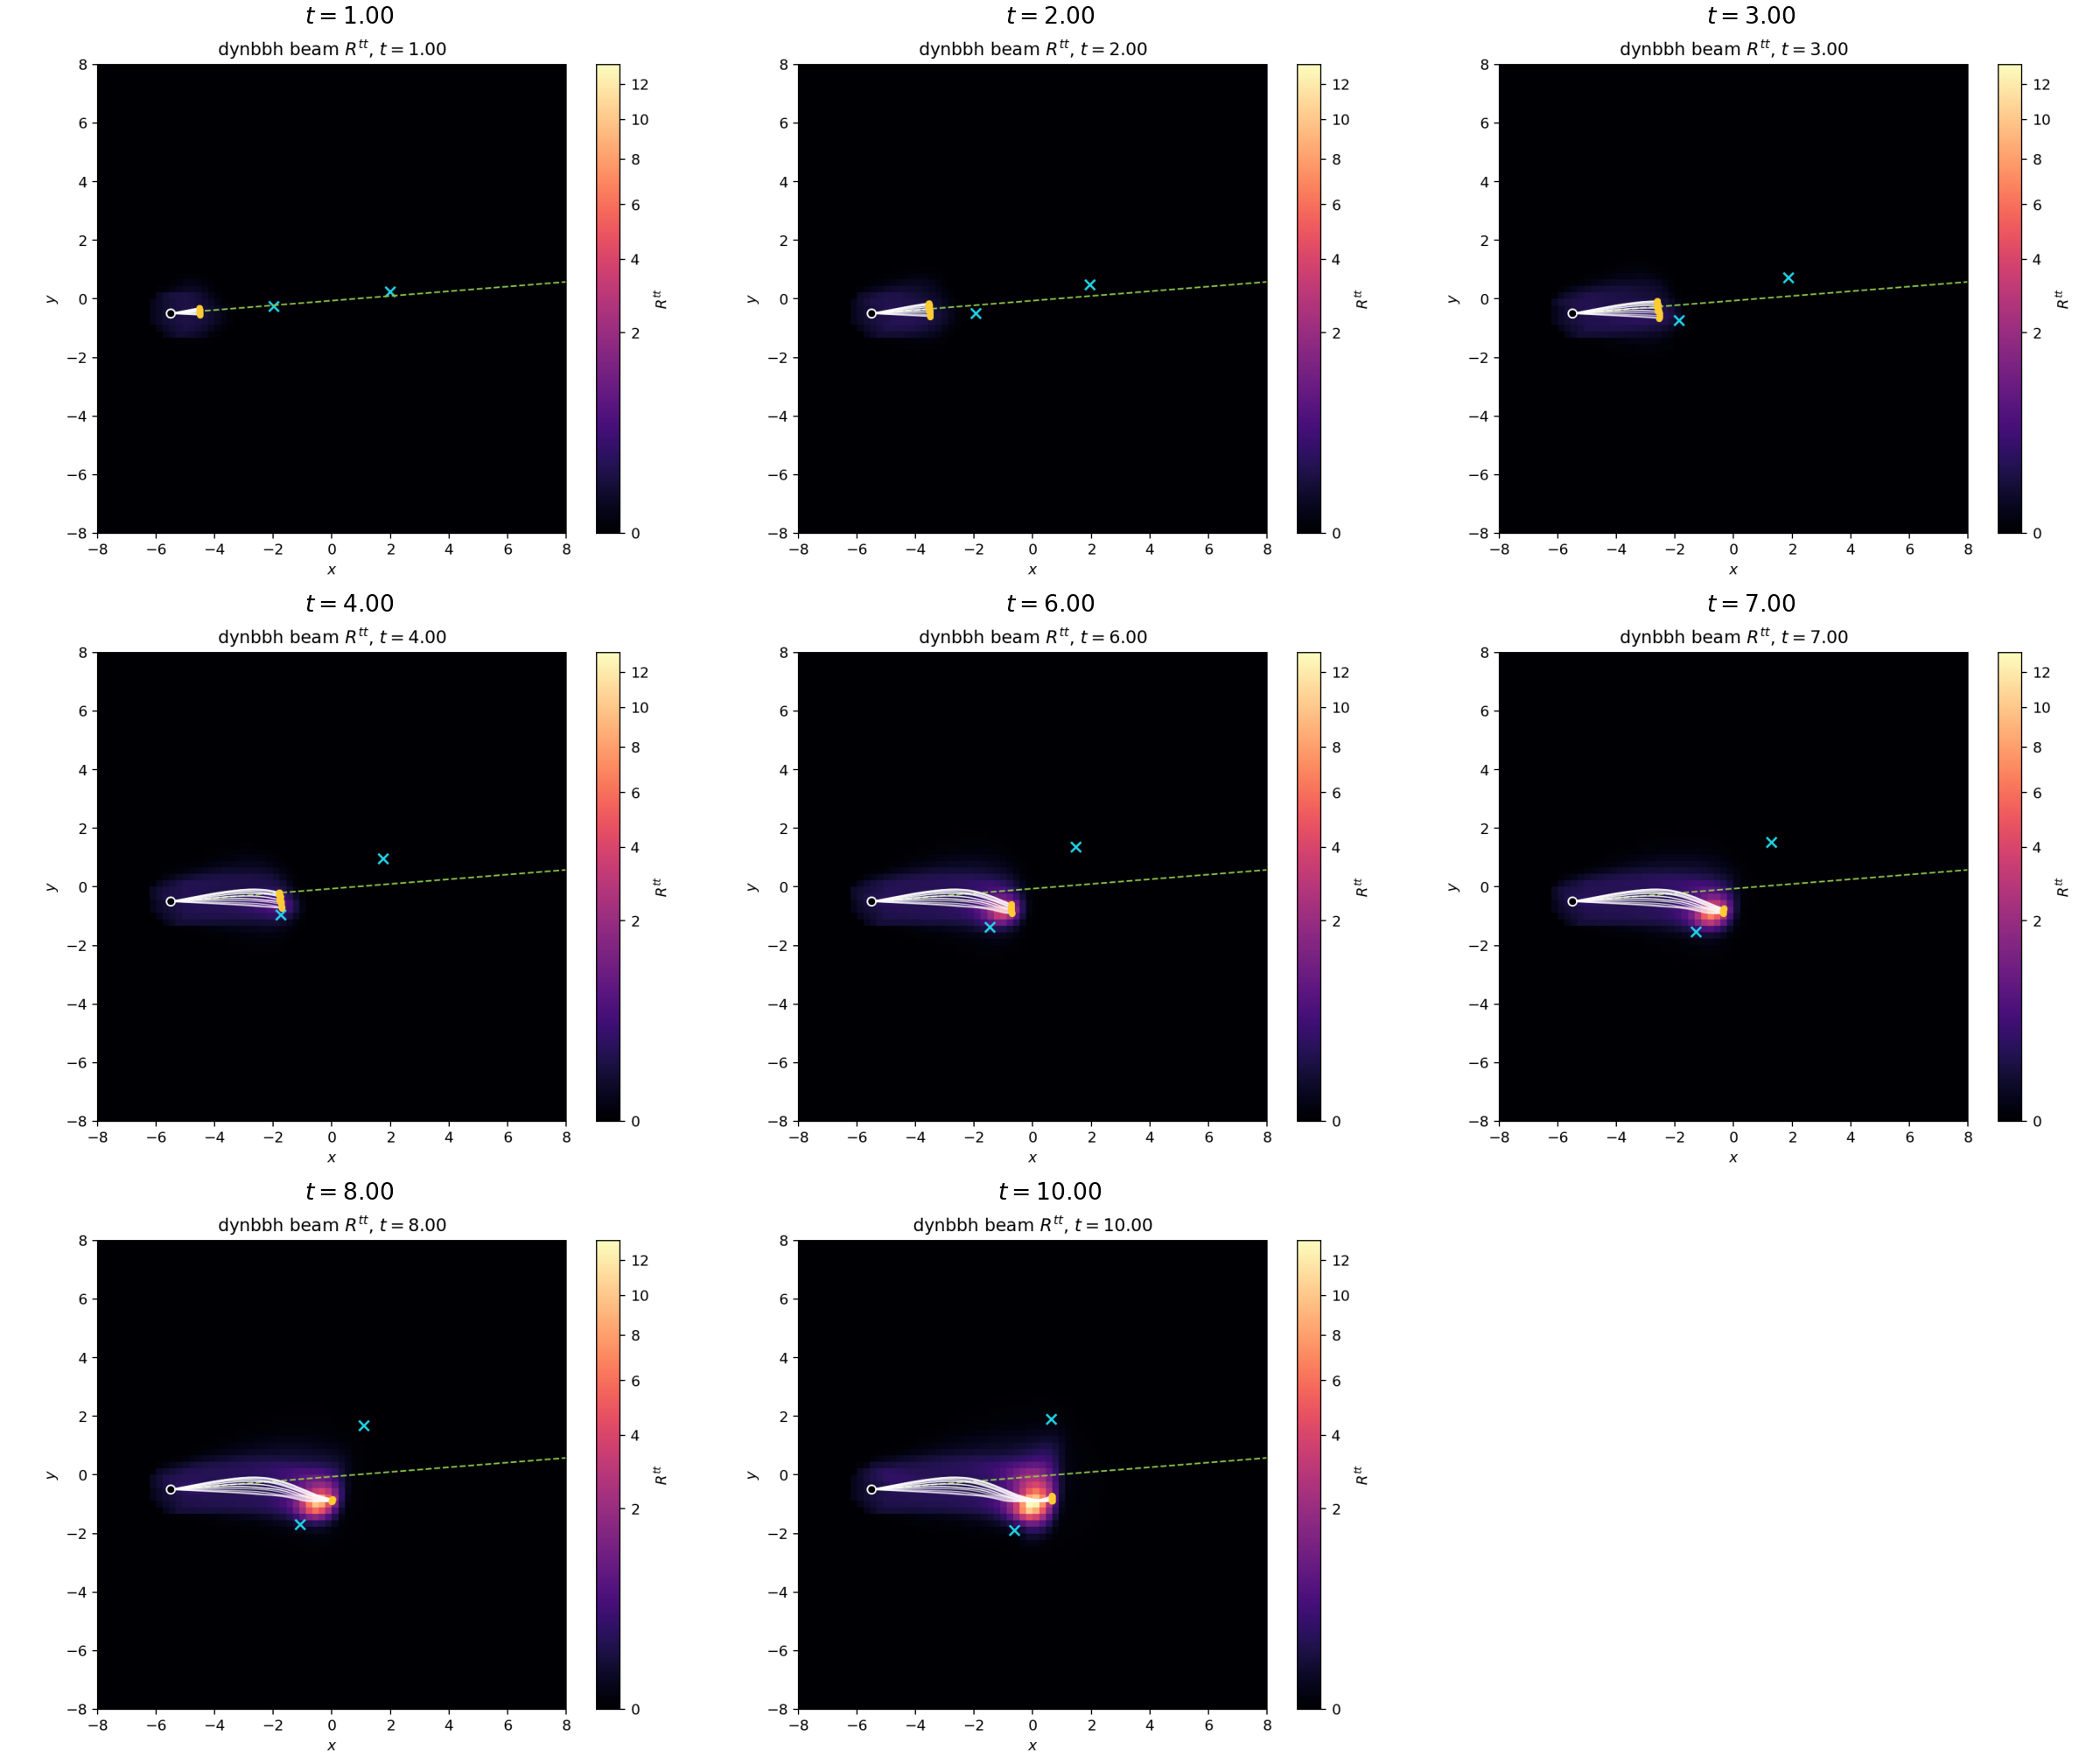
\includegraphics[width=0.98\linewidth]{figures/dynbbh_beam_timeseries.png}
\caption{High-resolution dynbbh ADM beam time series.  Each panel shows the
\(x-y\) slice of \(R^{tt}\) with the accumulated null-particle trajectories
overplotted through that output time.  The binary centers rotate according to
the superposed orbiting Kerr-Schild background used to populate the analytic
ADM fields.}
\label{fig:dynbbhtimeseries}
\end{figure}

\begin{figure}[htbp]
\centering
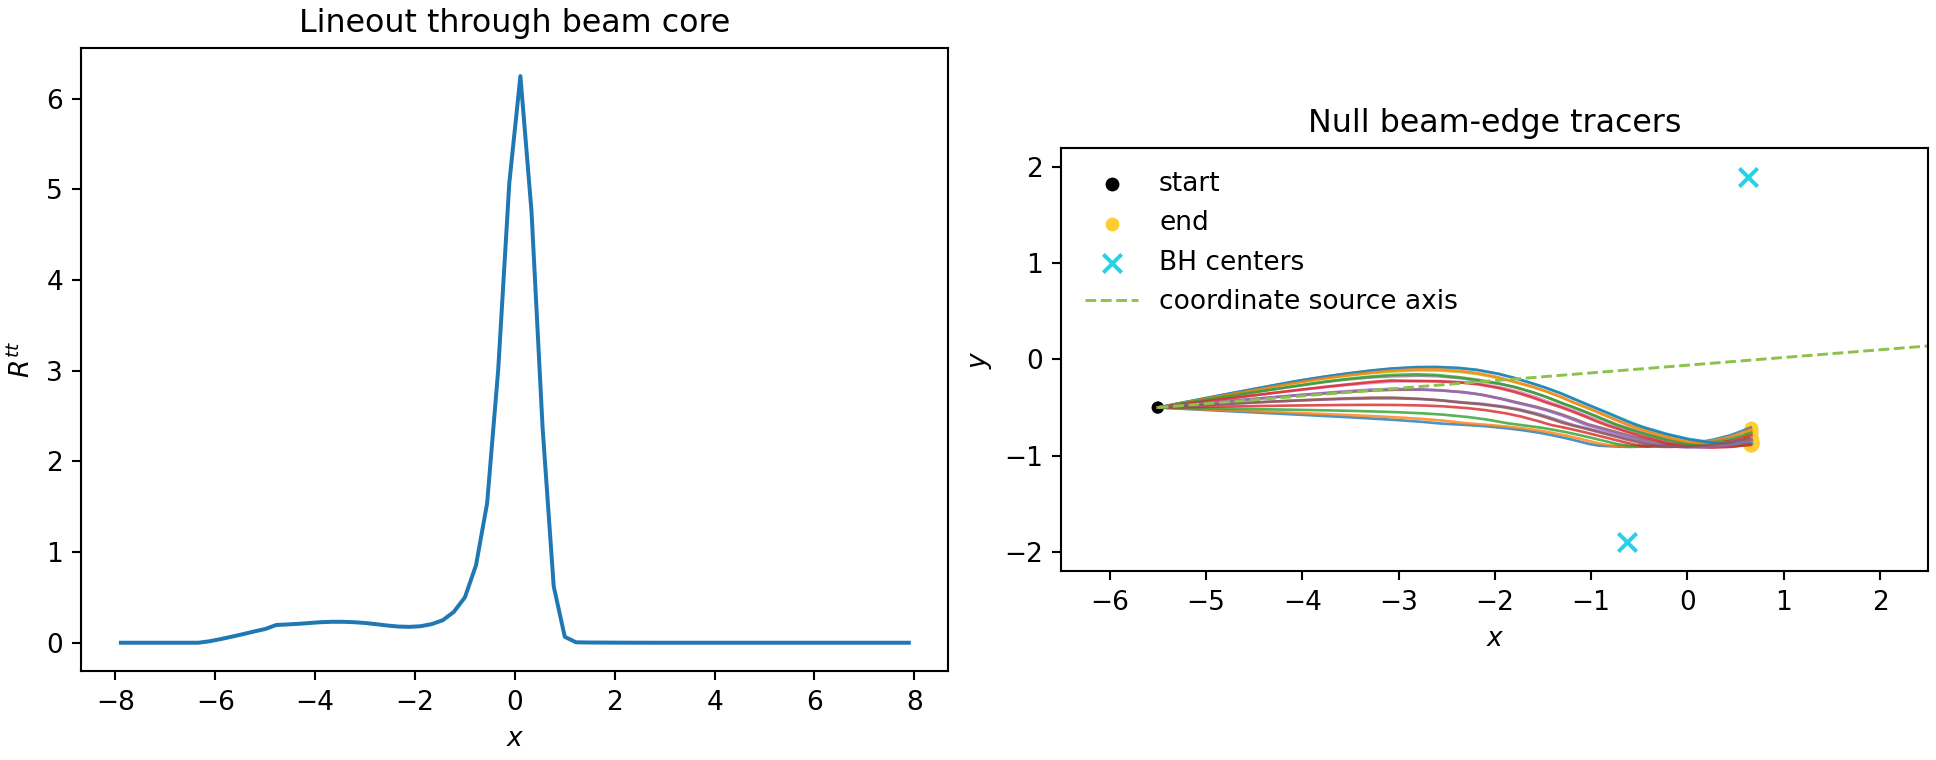
\includegraphics[width=0.92\linewidth]{figures/dynbbh_beam_particles_lineout.png}
\caption{Beam-core \(R^{tt}\) lineout and null beam-edge particle tracks for
the same compact dynbbh figure run.}
\label{fig:dynbbhlineout}
\end{figure}

\subsection{Diagnostic artifacts}

All diagnostic figures in this section are generated from committed inputs and
scripts.  Table~\ref{tab:plots} lists the plot artifacts, their producers, and
the numerical behavior each one is intended to check.

\begin{table}[htbp]
\centering
\footnotesize
\begin{tabular}{p{0.34\linewidth}p{0.25\linewidth}p{0.30\linewidth}}
\toprule
Figure file & Producer & Diagnostic \\
\midrule
\path{figures/beam_comparison.png} & \path{plot_comparisons.py} & 1D flat beam agreement across legacy CKS, dyn CKS, and dyn ADM-flat \\
\path{figures/beam_2d_fields.png} & \path{plot_comparisons.py} & 2D flat beam morphology in the same three branches \\
\path{figures/beam_2d_residuals.png} & \path{plot_comparisons.py} & residual maps against the legacy flat beam \\
\path{figures/linear_wave_errors.png} & \path{plot_comparisons.py} & final scalar error row for the CKS linear wave \\
\path{figures/linear_wave_convergence.png} & \path{run_linear_wave_convergence.py} & coupled fluid/radiation linear-wave convergence for legacy CKS, dyn CKS, and analytic-flat dyn ADM \\
\path{figures/crossing_beams_comparison.png} & \path{run_crossing_beams.py} & free streaming through crossing beams for legacy CKS, dyn CKS, dyn ADM-flat, and the analytic solution \\
\path{figures/crossing_beams_convergence.png} & \path{run_crossing_beams.py} & angular convergence for crossing beams in all three branches \\
\path{figures/kerr_orbit_beam_comparison.png} & \path{run_kerr_orbit_beam.py} & compact Kerr photon-orbit beam bending, including analytic ADM Kerr-Schild transport \\
\path{figures/equilibration_comparison.png} & \path{run_equilibration.py} & homogeneous gas-radiation relaxation against the exact ODE \\
\path{figures/adm_formal_tests.png} & \path{run_adm_formal_tests.py} & FLRW redshift, static lapse-gradient source, and ADM momentum-source closure \\
\path{figures/dynbbh_beam_particles.png} & \path{run_dynbbh_beam_figures.py} & ADM BBH beam source and null-particle beam-edge diagnostic \\
\path{figures/dynbbh_beam_rtt_slices.png} & \path{run_dynbbh_beam_figures.py} & \(R^{tt}\) beam slices on the superposed orbiting Kerr-Schild background \\
\path{figures/dynbbh_beam_adm_background.png} & \path{run_dynbbh_beam_figures.py} & ADM lapse and conformal-factor contours for the same binary slice \\
\path{figures/dynbbh_beam_particles_lineout.png} & \path{run_dynbbh_beam_figures.py} & beam-core lineout and null beam-edge tracers \\
\path{figures/dynbbh_beam_summary.png} & \path{run_dynbbh_beam_figures.py} & combined dynbbh beam/background/tracer diagnostic \\
\path{figures/dynbbh_beam_timeseries.png} & \path{run_dynbbh_beam_figures.py} & high-resolution dynbbh time-series snapshots with accumulated null-particle tracks \\
\bottomrule
\end{tabular}
\caption{Diagnostic plot artifacts for the standalone dynamical radiation
validation suite.}
\label{tab:plots}
\end{table}

\begin{table}[htbp]
\centering
\small
\begin{tabular}{p{0.30\linewidth}p{0.38\linewidth}p{0.20\linewidth}}
\toprule
Test & Quantity checked & Result \\
\midrule
Flat beam, CKS compatibility & \(\max |R^{00}_{\rm dynrad}-R^{00}_{\rm legacy}|\) & \(0\) \\
Flat beam, ADM mode & \(\max |R^{00}_{\rm ADM}-R^{00}_{\rm legacy}|\) & \(0\) \\
Flat ADM beam, MPI & two-rank decomposition & passed \\
Stationary KS ADM beam & nonzero ADM angular drift & passed \\
Dynamic Z4c ADM smoke & time-dependent ADM metric cache & passed \\
CKS linear wave & final error row & identical \\
CKS/ADM linear-wave convergence & fluid and radiation moment errors versus analytic eigenmode & legacy/dyn CKS/dyn ADM overlap; RMS rate \(2.07\) \\
Crossing beams & free-streaming through another beam and angular convergence & source-aligned from \(N_{\rm ang}=12\); ADM-CKS \(L_\infty \le 4.3\times10^{-4}\) \\
Kerr photon-orbit beam & stationary Kerr bending on an \(n_{x_3}=1\) grid & legacy, CKS, and ADM ridges follow orbit; ADM-CKS \(L_\infty=4.50\times10^{-2}\) \\
Gas-radiation equilibration & homogeneous source relaxation and total-energy conservation & final legacy/dyn states identical; \(u_{\rm tot}=4\) \\
FLRW ADM redshift & homogeneous \(E\propto a^{-4}\), \(\sqrt{\gamma}E\propto a^{-1}\) & final relative errors \(1.19\times10^{-4}\) \\
Static lapse-gradient source & sign and shape of \(-F^i\partial_i\alpha\) & correlation \(0.999307\), relative RMS \(4.68\times10^{-2}\) \\
ADM momentum-source closure & Hamiltonian force sum versus Valencia momentum source & absolute residual \(1.15\times10^{-6}\) at \(N_x=128\) \\
Positivity limiter & angular zeroth-moment preserving redistribution (CKS and ADM) & passed \\
Iterated source solve & temperature-dependent fixed-fluid coupling & passed \\
Restart & write and resume \code{dynrad\_beam\_cks} & passed \\
Z4c CKS rejection & unsupported metric mode guard & passed \\
BBH legacy radiation rejection & \code{prad} guard & passed \\
BBH ADM beam & finite beam and real source-rank particle tracks & passed in four-rank MPI to \(t=10\) \\
BBH ADM coupling & absorption/scattering with MHD primitives & passed in serial \\
BBH coupled MPI smoke & two-rank dynbbh/MHD run & passed \\
\bottomrule
\end{tabular}
\caption{Current regression status for the standalone dynamical radiation
implementation.}
\label{tab:tests}
\end{table}

\section{Comparison With the Existing Solver}
\label{sec:comparison}

\begin{table}[htbp]
\centering
\small
\begin{tabular}{p{0.25\linewidth}p{0.31\linewidth}p{0.31\linewidth}}
\toprule
Feature & \code{radiation} & \code{dyn\_radiation} \\
\midrule
Metric source & Analytic stationary CKS metric & CKS compatibility mode or ADM mesh fields \\
Conserved intensity & signed \(k^0k_0I\) & CKS: signed \(k^0k_0I\); ADM: \(\sqrt{\gamma}I\) \\
Spatial speed & \(k^i/k^0\) from stationary tetrad & CKS: \(k^i/k^0\); ADM: \(\alpha s^i-\beta^i\) \\
Metric source terms & Stationary tetrad and angular drift coefficients & ADM Valencia energy source using \(K_{ij}\) and \(\partial_i\alpha\) \\
Angular bending & Precomputed CKS coefficients & Cached ADM Hamiltonian angular drift \\
Matter coupling & Existing local implicit path & CKS path retained; ADM uses \(I=U/\sqrt{\gamma}\), Eulerian tetrad frequency, and Valencia moment feedback \\
Metric backreaction & Not applicable to fixed metric & Not included; radiation is metric-passive \\
Binary backgrounds & Not supported directly & Supported through ADM fields \\
\bottomrule
\end{tabular}
\caption{Functional comparison between the existing stationary radiation solver
and the new standalone dynamical-background solver.}
\label{tab:comparison}
\end{table}

The key mathematical difference is the removal of the signed stationary-metric
normalization in ADM mode.  The key implementation difference is that metric
data are no longer assumed to be analytic or time independent.  The new solver
therefore fits the same design pattern as the Valencia GRMHD path: fluxes and
sources are built from ADM variables supplied by the active spacetime module.
At present this analogy is limited to transport and matter coupling.  The
radiation stress-energy tensor is not passed to the metric solver, so Z4c
evolutions see MHD/dynGRMHD matter sources only.

\section{How to Check the Formalism}
\label{sec:checklist}

The derivation above gives several concrete checks that can be applied to the
implementation.

\paragraph{Flat-space limit.}
Set \(\alpha=1\), \(\beta^i=0\), \(\gamma_{ij}=\delta_{ij}\), and
\(K_{ij}=0\).  Then \(E^i_{\ (\hat a)}=\delta^i_{\hat a}\),
\(U_n=I_n\), \(v^i=s^i\), \(S_n^{\rm geom}=0\), and all angular drift
coefficients vanish.  The ADM solver must reduce to ordinary Cartesian
free-streaming.  This is the reason the flat ADM beam can match the legacy
flat CKS beam exactly.

\paragraph{Moment-source check.}
For any angular distribution, compute the discrete moments in
Equation~\eqref{eq:moments}.  The angular sum of the per-angle energy source
in Equation~\eqref{eq:anglesource} must equal the right-hand side of
Equation~\eqref{eq:valenciaE}.  The automated
\code{rad\_momentum\_source} regression now performs the stronger local check
that the angular Hamiltonian force sum produces the Valencia momentum source
in Equation~\eqref{eq:valencia_momentum}.  The residual is expected to be
second order in the ADM metric-gradient cache spacing because
\(\partial_j\gamma_{ik}\) and \(\partial_j\gamma^{ik}\) are independently
finite-differenced.

\paragraph{ADM redshift checks.}
The \code{rad\_flrw\_redshift} regression verifies the sign of the
\(\alpha K_{ij}s^is^j\) source by checking \(E\propto a^{-4}\) and
\(\sqrt{\gamma}E\propto a^{-1}\).  The \code{rad\_lapse\_gradient}
regression verifies the sign of \(-s^i\partial_i\alpha\) by comparing a short
anisotropic run against the first-order lapse-gradient source prediction.

\paragraph{Tetrad consistency check.}
At every cached cell,
\begin{equation}
  \gamma_{ij}E^i_{\ (\hat a)}E^j_{\ (\hat b)}
  =\delta_{\hat a\hat b},\qquad
  e^{(\hat a)}_{\ i}E^i_{\ (\hat b)}
  =\delta^{\hat a}_{\ \hat b}.
\end{equation}
The same Cholesky gauge must be used for spatial transport, angular drift, and
matter coupling; otherwise spurious angular drift appears even in locally flat
coordinates.

\paragraph{Frequency-transform check.}
For a fluid comoving with the Eulerian observer,
\(u^{(\hat0)}=1\) and \(u^{(\hat a)}=0\), so
\(D=\nucm/\nuE=1\).  The ADM coupling must then use
\(I_{\rm cm}=U/\sqrt{\gamma}\).  For a moving fluid, the fourth-power intensity
transform and the inverse-square solid-angle transform in
Equation~\eqref{eq:intensity_angle_transform} must be applied together; using
one without the other gives the wrong comoving mean intensity.

\paragraph{Local conservation check.}
When \code{affect\_fluid=true}, the matter-coupling kernel should change gas
energy and momentum by the negative of the change in the radiation moments in
Equation~\eqref{eq:adm_feedback_moments}.  This is independent of how the
implicit temperature solve is performed.

\section{Discussion and Limitations}
\label{sec:discussion}

The present implementation is a controlled step toward dynamical radiation
transport.  It moves radiation energy on ADM backgrounds, bends the angular
directions with an ADM Hamiltonian operator, reproduces stationary beam and
linear-wave regressions, and diagnoses beam propagation on the superposed binary
metric.  It is still not a final production radiation module.  The current
coupling to dynamical spacetime is one-way: ADM/Z4c geometry drives radiation,
but radiation does not feed \(T_{\mu\nu}\) back into the Z4c right-hand side.
The angular
operator uses second-order metric-gradient caches; higher-order gradients and
limiters can be added behind the same cache interface.  The local
momentum-source consistency check in Equation~\eqref{eq:valencia_momentum} is
now included in the regression suite; broader momentum-balance tests on
genuinely time-dependent ADM backgrounds remain future validation work.

The ADM matter-coupling path now uses the Eulerian tetrad frequency factor,
\(I=U/\sqrt{\gamma}\), and gas feedback through the Valencia radiation moments.
It has passed flat and BBH smoke tests, a homogeneous gas-radiation relaxation
comparison against the exact source ODE, and a temperature-dependent
fixed-fluid source iteration test.  It still needs a broader validation suite
with moving-fluid absorption/scattering, optically thick diffusion, and
time-dependent metric backgrounds.  The ADM metric source is now applied with
the exponential source increment in Equation~\eqref{eq:geom_exp_update}.  The
transport and source updates use the zeroth-moment-conserving angular
positivity limiter described above; production diagnostics should still count
limiter activations so runs can identify under-resolved optically thin
features.

The changed kernels were reviewed for Kokkos device compatibility: the stage
geometry cache, timestep reductions, fluxes, and coupling kernels capture only
device views and POD scalars, and device-side finiteness tests use
\code{Kokkos::isfinite}.  The tests reported here were run on the local CPU/MPI
builds.  No CUDA, HIP, or SYCL runtime validation was available in this pass,
so GPU execution should be treated as statically reviewed but not
runtime-certified.

Finally, the null-particle pusher is currently a diagnostic tool.  It uses
nearest-cell ADM fields and centered finite differences.  It is useful for beam
edge visualization and for catching obvious metric or sign errors.  Its
timestep cap uses the ADM coordinate light-speed bound
\(|\beta^q|+\alpha\sqrt{\gamma^{qq}}\), so it respects shifted and small-lapse
coordinates during particle boundary exchange.  A scientific geodesic
integrator should still use higher-order metric interpolation, adaptive
timestepping, and a stricter monitor of the null Hamiltonian.

\section{Conclusions}
\label{sec:conclusions}

We implemented and documented a standalone dynamical-background radiation
module for AthenaK.  The solver preserves the legacy CKS variables and flat
regression behavior in a compatibility mode and adds an ADM mode based on
Eulerian densitized intensity, Valencia
coordinate speeds, and a per-angle geometric source whose angular sum recovers
the Valencia radiation energy equation.  The formulation is suitable for
time-dependent ADM backgrounds because metric evolution enters through
\(K_{ij}\) and the ADM co-triad time derivative, rather than through
stationarity assumptions.  Regression tests show exact agreement with the
legacy flat beam, identical stationary CKS linear-wave error norms, successful
two-rank flat ADM beam transport, excision-safe stationary black-hole ADM
timesteps, homogeneous gas-radiation equilibration against the exact source
ODE, ADM FLRW redshift, ADM lapse-gradient and momentum-source closure checks,
restart coverage, and serial plus two-rank ADM beam/null-particle smoke tests
on the superposed binary black-hole background.  The remaining work is to add
radiation metric backreaction, extend ADM validation to moving-fluid and fully
time-dependent metric problems, add runtime diagnostics for positivity-limiter
activation, and upgrade the diagnostic particle pusher if high-accuracy
geodesics are required.

\end{document}
